\documentclass[11pt,a4paper]{article}
\usepackage[english]{babel}
\usepackage[utf8]{inputenc}
\usepackage[T1]{fontenc}
\usepackage{csquotes}
\usepackage{geometry}
\usepackage{microtype}
\usepackage{hyperref}
\usepackage{graphicx}
\usepackage{caption}
\usepackage{subcaption}
\usepackage{enumitem}
\usepackage{longtable}
\usepackage{booktabs}
\usepackage{amsmath}
\usepackage{float}
\usepackage{tabularx}
\usepackage{xcolor}
\usepackage{tcolorbox}
\tcbuselibrary{listings, minted, skins, breakable}

% Stile personalizzato per i blocchi SQL
\newtcblisting{sqlbox}[2][]{
  listing engine=minted,
  minted language=sql,
  minted style=colorful,
  minted options={fontsize=\small, breaklines, autogobble, linenos=false},
  colback=blue!5!white,
  colframe=blue!50!black,
  coltitle=white,
  title=#2,
  fonttitle=\bfseries,
  listing only,
  breakable,
  enhanced,
  #1
}

\geometry{margin=2.5cm}

\begin{document}

% Custom title page
\begin{titlepage}
	\centering
	
	% Logo UniBa (se hai il file logo.png nella cartella img/)
	\vspace*{1cm}
	
\includegraphics[width=0.3\textwidth]{img/logo_uniba.png}
	
	\vspace{1.5cm}
	
	{\LARGE \textbf{University of Bari Aldo Moro}}\\[0.5cm]
	{\Large Computer Science Department}
	
	\vspace{2cm}
	
	{\huge \textbf{WHO Disease Monitoring System}}\\[0.3cm]
	{\Large Database Systems Project Work}
	
	\vfill
	
	\begin{minipage}{0.45\textwidth}
		\begin{flushleft}
			\textbf{Student:}\\
			Mauro Carlucci\\
			830627\\
			\href{mailto:m.carlucci66@studenti.uniba.it}{m.carlucci66@studenti.uniba.it}
		\end{flushleft}
	\end{minipage}
	\hfill
	\begin{minipage}{0.45\textwidth}
		\begin{flushright}
			\textbf{Professor:}\\
			Paolo Mignone\\
			\href{mailto:paolo.mignone@uniba.it}{paolo.mignone@uniba.it}
		\end{flushright}
	\end{minipage}
	
	\vspace{1.5cm}
	
	{\large Academic Year 2024/2025}\\[0.3cm]
	{}
	
\end{titlepage}

\tableofcontents
\newpage

\section{Requirements Collection}
\label{sec:req-collection}
	\textbf{Specifics.}\\
\emph{``The "WHO" organization has implemented a system for monitoring diseases with detailed descriptions. The system allows WHO storing biological data that could refer to tissues or organs with their description. Specifically, the tissues and organs are described through the donor details, a general condition (control, disease) and, when affected, the specific disease. Furthermore, the system saves the organ/tissue name, textual description, position within the human body, density, if it is required for life (e.g., the brain, the heart and so on). The donors are described through name, surname, date of birth, age, sex. The company has the storage about the diseases and their descriptions: name, discovery date and time, and textual description, whether it is treatable or not, the possible cure. A cure is described with a treatment, a list of drugs to be taken, while the drugs have the name, description, a percentage of success for a specific disease, a list of possible allergies linked to such a drug. For each organ/tissue, the system saves the sequence of treatments with specific drugs and the effects observed. For each positive observed effect, the system could suggest a possible new cure/treatment to be investigated and it suggests possible future works to the list of researchers registered. The system maintains the information of the registered researchers. Specifically, it saves the name, surname, list of publications. A publication is described via a DOI identifier, title, journal, or conference with a degree of quality (top, middle, low).''}

\section{Requirements Analysis}

\subsection{Choosing the correct level of abstraction}

At line 2, the description of biological data is general, since it may refer either to tissues or organs. Therefore, we assume that a biological data entry is classified as either \textit{tissue} or \textit{organ}, and for each of them the following details are stored: id, name, textual description, position within the human body, density, and whether it is required for life (e.g., brain, heart).

At line 3, the description of tissues and organs refers to donor details. We assume that each donor is described through: name, surname, date of birth, age, sex, and a unique CF identifier.

At line 4, the condition of a tissue/organ is described as general (control or disease). We assume that for each biological data entry there is a condition attribute that can be either \textit{control} or \textit{disease}. In case of \textit{disease}, the biological data entry references a specific disease.

At line 5, the system stores diseases with a general description. We assume that each disease is characterized by: id, name, discovery date, textual description, and whether it is treatable or not.

At line 6, the requirement states that a cure is defined as a treatment. Since no specific distinction is provided between the two concepts, we assume that \textit{cure} and \textit{treatment} refer to the same entity. Each treatment is characterized by: id, name, and a description.

At line 7, the drugs are described in a general manner. Therefore, we assume that each drug is characterized by: id, name, description, and a percentage of success for a specific disease. Drugs may cause allergies.

At line 8, the requirement refers to allergies but does not specify their details. We assume that each allergy is characterized by: id, name, and description.

At line 10, the requirement specifies that positive observed effects may suggest possible new cures or treatments to be investigated. We assume that these \textit{future works} are represented as proposals generated from positive treatments. Each future work is characterized by: id, title, and textual description.

At line 11, the system maintains registered researchers. We assume that each researcher is described by: name, surname, and a unique CF identifier.

At line 12, publications are described in a general way. We assume that each publication is characterized by: DOI identifier, title, publisher (journal or conference), and a quality level (\textit{top}, \textit{middle}, \textit{low}).

\subsubsection{Output}

The ``WHO'' organization has implemented a system for monitoring diseases with detailed descriptions. The system manages biological data classified as either organs or tissues. Each biological data entry is characterized by: id, name, textual description, position within the human body, density, and whether it is required for life. Each organ or tissue is associated with a donor, characterized by name, surname, date of birth, age, sex, and a CF identifier, and with a condition that can be \textit{control} or \textit{disease}. If the condition is \textit{disease}, the biological data entry references a specific disease.

Each disease is characterized by: id, name, discovery date, description, and treatability. For every disease, one or more treatments may exist. A treatment is described by: id, name, and description, and is composed of one or more drugs. Drugs are characterized by: id, name, description, success percentage, and possible related allergies. Allergies are described by: id, name, and description.

For each organ or tissue, the system records a sequence of treatments. A treatment applied to a disease is characterized by: id, date, effect description, and outcome (positive or negative). When positive effects are observed, the system may generate \textit{future works} to be considered for further investigation. Each future work has an id, a title, and a description.

Researchers are maintained in the system and are characterized by: name, surname, and a CF identifier. Each researcher may be associated with future works and produces publications. A publication is characterized by: DOI identifier, title, publisher (journal or conference), and a quality level (\textit{top}, \textit{middle}, \textit{low}).

\subsection{Standardize sentence structure}

\begin{tabularx}{\textwidth}{|X|X|}
\hline
\textbf{Main sentence} & \textbf{Sentence transformed} \\
\hline
The ``WHO'' organization has implemented a system for monitoring diseases with detailed descriptions. &
The ``WHO'' organization manages a system for monitoring diseases. \\
\hline
The system manages biological data classified as either organs or tissues. Each biological data entry is characterized by: id, name, textual description, position within the human body, density, and whether it is required for life. &
The system manages biological data. For biological data, we handle the id, name, textual description, position, density, and life requirement. Biological data can be classified as either organ or tissue. \\
\hline
Each organ or tissue is associated with a donor, characterized by name, surname, date of birth, age, sex, and a CF identifier, and with a condition that can be \textit{control} or \textit{disease}. If the condition is \textit{disease}, the biological data entry references a specific disease. &
Each organ or tissue is associated with a donor. For donor, we handle the name, surname, date of birth, age, sex, and CF identifier. For biological data, we handle the condition that can be \{control, disease\}. If condition is disease, the biological data references a disease. \\
\hline
Each disease is characterized by: id, name, discovery date, description, and treatability. For every disease, one or more treatments may exist. &
For disease, we handle the id, name, discovery date, description, treatability. Each disease may have one or more treatments. \\
\hline
A treatment is described by: id, name, and description, and is composed of one or more drugs. Drugs are characterized by: id, name, description, success percentage, and possible related allergies. Allergies are described by: id, name, and description. &
For treatment, we handle the id, name, description. Each treatment is composed of one or more drugs. For drug, we handle the id, name, description, success percentage. For allergy, we handle the id, name, description. \\
\hline
For each organ or tissue, the system records a sequence of treatments. A treatment applied to a disease is characterized by: id, date, effect description, and outcome (positive or negative). &
For organ or tissue, the system records a sequence of treatments. For applied treatment, we handle the id, date, effect description, and outcome \{positive, negative\}. \\
\hline
When positive effects are observed, the system may generate \textit{future works} to be considered for further investigation. Each future work has an id, a title, and a description. &
When positive effects are observed, the system generates future works. For future work, we handle the id, title, description. \\
\hline
Researchers are maintained in the system and are characterized by: name, surname, and a CF identifier. Each researcher may be associated with future works and produces publications. &
For researcher, we handle the name, surname, CF identifier. Researchers can be associated with future works and produce publications. \\
\hline
A publication is characterized by: DOI identifier, title, publisher (journal or conference), and a quality level (\textit{top}, \textit{middle}, \textit{low}). &
For publication, we handle the DOI identifier, title, publisher, and quality level \{top, middle, low\}. \\
\hline
\end{tabularx}

\subsubsection{Output}

The ``WHO'' organization manages a system for monitoring diseases. The system manages biological data. For biological data, we handle the id, name, textual description, position, density, and life requirement. Biological data can be classified as either organ or tissue. Each organ or tissue is associated with a donor. For donor, we handle the name, surname, date of birth, age, sex, and CF identifier. For biological data, we handle the condition that can be \{control, disease\}. If condition is disease, the biological data references a disease. For disease, we handle the id, name, discovery date, description, treatability. Each disease may have one or more treatments. For treatment, we handle the id, name, description. Each treatment is composed of one or more drugs. For drug, we handle the id, name, description, success percentage. For allergy, we handle the id, name, description. For organ or tissue, the system records a sequence of treatments. For applied treatment, we handle the id, date, effect description, and outcome \{positive, negative\}. When positive effects are observed, the system generates future works. For future work, we handle the id, title, description. For researcher, we handle the name, surname, CF identifier. Researchers can be associated with future works and produce publications. For publication, we handle the DOI identifier, title, publisher, and quality level \{top, middle, low\}.

\subsection{Identification of synonyms and homonyms and resolving complex phrases}

At a certain point we noticed that in the extract a publication can be associated either with a \textit{journal} or a \textit{conference}.  
This makes the term ambiguous, therefore we decided to replace both \textit{journal} and \textit{conference} with the unique term \textit{publisher}.  

We also observed that the extract uses both the terms \textit{cure} and \textit{treatment}.  
Since they do not introduce any semantic distinction, we decided to keep only the term \textit{treatment}.  

After the identification and resolution of these homonyms we also resolved complex phrases.

\subsubsection{Output}

The ``WHO'' organization manages a system for monitoring diseases.  
The system manages biological data. For biological data, we handle the id, name, textual description, position, density, and life requirement. Biological data can be classified as either organ or tissue.  

Each organ or tissue is associated with a donor. For donor, we handle the name, surname, date of birth, age, sex, and CF identifier. For biological data, we handle the condition that can be \{control, disease\}. If condition is disease, the biological data references a disease.  

For disease, we handle the id, name, discovery date, description, treatability. Each disease may have one or more treatments.  
For treatment, we handle the id, name, description. Each treatment is composed of one or more drugs.  
For drug, we handle the id, name, description, success percentage.  
For allergy, we handle the id, name, description.  

For organ or tissue, the system records a sequence of treatments. For applied treatment, we handle the id, date, effect description, and outcome \{positive, negative\}.  
When positive effects are observed, the system generates future works. For future work, we handle the id, title, description.  

For researcher, we handle the name, surname, CF identifier. Researchers can be associated with future works and produce publications.  
For publication, we handle the DOI identifier, title, publisher, and quality level \{top, middle, low\}.

\subsection{Glossary of Terms}

\begin{tabular}{|p{3cm}|p{7cm}|p{3cm}|p{3cm}|}
\hline
\textbf{Concept} & \textbf{Description} & \textbf{Synonym} & \textbf{Link} \\
\hline
Biological Data & Represents an organ or tissue, characterized by structural and descriptive attributes & Organ, Tissue & Donor, Condition, Disease \\
\hline
Donor & Person associated with an organ or tissue, providing personal and identification data & -- & Biological Data \\
\hline
Condition & State of biological data, which can be \{control, disease\} & -- & Biological Data, Disease \\
\hline
Disease & Medical condition associated with biological data, characterized by identification and description & -- & Biological Data, Treatment \\
\hline
Treatment & Medical intervention applied to a disease, can consist of one or more drugs & Cure & Disease, Drug \\
\hline
Drug & A medicine used within a treatment, characterized by success rate and possible allergies & -- & Treatment, Allergy \\
\hline
Allergy & Negative reaction related to a drug & -- & Drug \\
\hline
Future Work & Research direction generated from positive outcomes of treatments & -- & Researcher \\
\hline
Researcher & Person in the system that can be associated with future works and publications & -- & Future Work, Publication \\
\hline
Publication & Scientific output produced by a researcher, published in a publisher with quality level & - & Researcher \\
\hline
\end{tabular}

\subsection{Phrases grouped by Concept}

\paragraph{Phrases related to Biological Data} 
The system manages biological data. For biological data, we handle the id, name, textual description, position, density, and life requirement. Biological data can be classified as either organ or tissue. For biological data, we handle the condition that can be \{control, disease\}. If condition is disease, the biological data references a disease. For organ or tissue, the system records a sequence of treatments.

\paragraph{Phrases related to Donor} 
Each organ or tissue is associated with a donor. For donor, we handle the name, surname, date of birth, age, sex, and CF identifier.

\paragraph{Phrases related to Disease} 
For disease, we handle the id, name, discovery date, description, treatability. Each disease may have one or more treatments.

\paragraph{Phrases related to Treatment} 
For treatment, we handle the id, name, description. Each treatment is composed of one or more drugs. For applied treatment, we handle the id, date, effect description, and outcome \{positive, negative\}.

\paragraph{Phrases related to Drug} 
For drug, we handle the id, name, description, success percentage. 

\paragraph{Phrases related to Allergy} 
For allergy, we handle the id, name, description.

\paragraph{Phrases related to Future Work} 
When positive effects are observed, the system generates future works. For future work, we handle the id, title, description.

\paragraph{Phrases related to Researcher} 
For researcher, we handle the name, surname, CF identifier. Researchers can be associated with future works and produce publications.

\paragraph{Phrases related to Publication} 
For publication, we handle the DOI identifier, title, publisher, and quality level \{top, middle, low\}.

\section{Conceptual Design}
\subsection{Skeleton Schema}

From the specifications, we read that biological data can refer to organs or tissues, which could naturally be translated in an ER diagram as a generalization. However, since the rest of the specifications do not imply any difference in attributes or relationships for organs versus tissues, it was decided to use only the single entity Biological Data.
The skeleton schema that outlines these entities and their main relationships is reported in Figure~\ref{fig:skeleton-schema}.
We will adopt a mixed strategy to make further refinements, carefully considering each step while analyzing the phrases grouped by concepts. This approach allows us to iteratively refine the schema by balancing both a top-down perspective and a bottom-up perspective.

\begin{figure}[H]
\centering
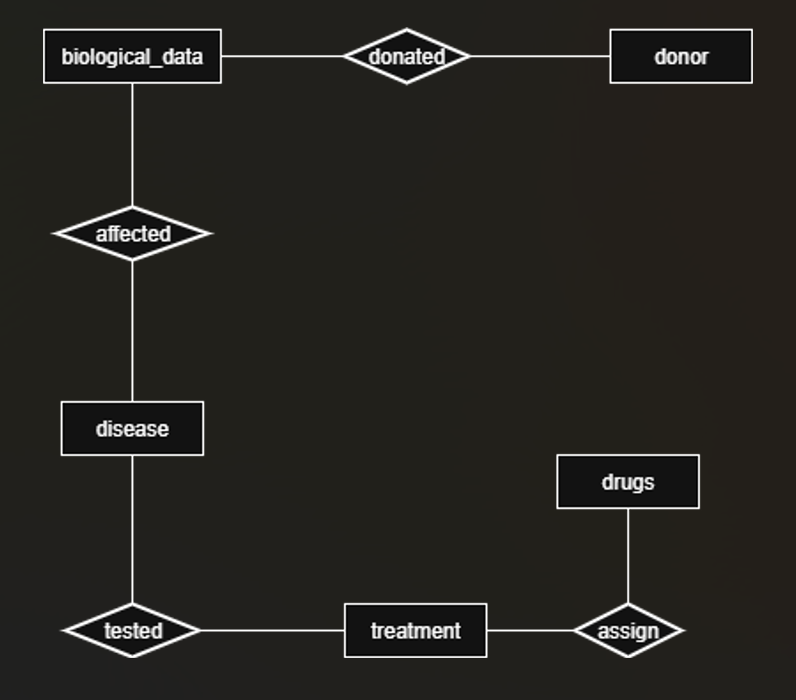
\includegraphics[width=0.55\textwidth]{img/skeleton.drawio.png}
\caption{Skeleton Schema representing the main entities of the system}
\label{fig:skeleton-schema}
\end{figure}

\subsection{Conceptual Schema}
The conceptual schema has been generated using a mixed strategy that combines both bottom-up and top-down refinements. The resulting model is shown in Figure~\ref{fig:conceptual-schema}.
During the design phase, a crucial modeling choice concerned the relationship between \textit{Disease}, \textit{Treatment}, and \textit{Future Work}. Initially, this was modeled as a ternary relationship, since a \textit{Future Work} can be proposed only as the result of a specific treatment applied to a disease. However, this direct ternary relationship was reified by introducing a new entity: \textit{Experiment}.
The \textit{Experiment} entity captures the application of a treatment to a disease for a specific organ or tissue, storing the observed effects and outcomes. This reification provides a clearer representation of the semantics:

\begin{itemize}
    \item \textit{Disease} and \textit{Treatment} are linked through the \textit{Experiment}.
    \item Each \textit{Experiment} has attributes such as id, date, effect description, and outcome (positive or negative).
    \item When the outcome is positive, the system may generate one or more \textit{Future Works} directly linked to the \textit{Experiment}.
\end{itemize}

This design choice improves extensibility and reduces ambiguity.

\begin{figure}[H]
\centering
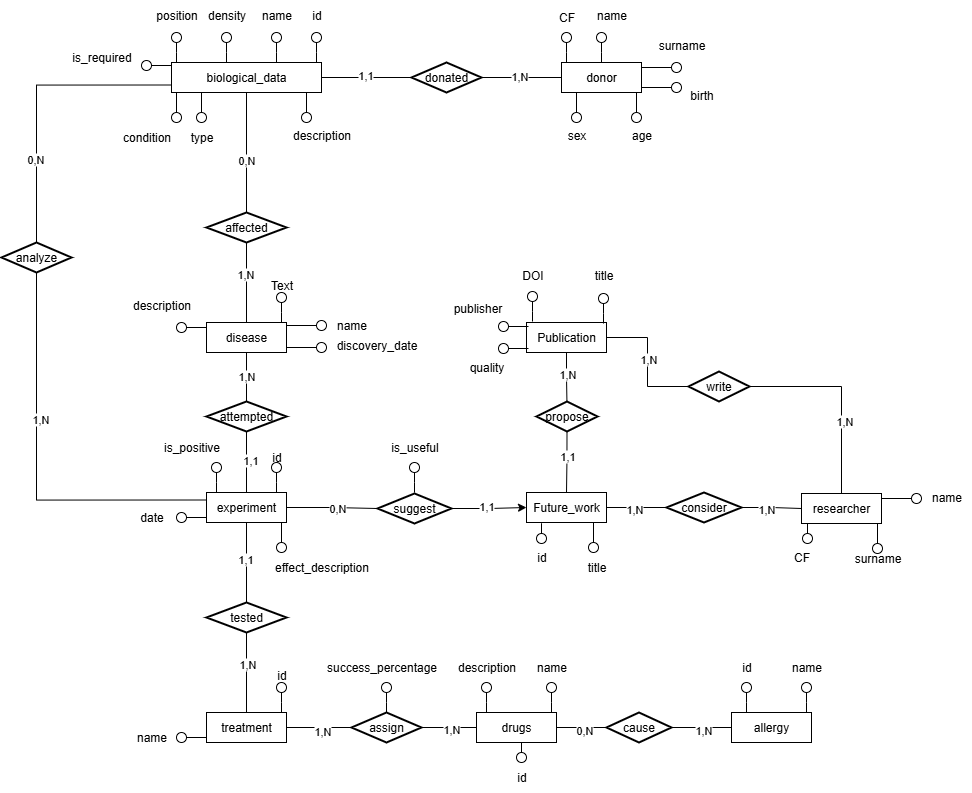
\includegraphics[width=1.1\textwidth]{img/Diagramma ER.drawio.png}
\caption{Conceptual Schema of the system after refinements}
\label{fig:conceptual-schema}
\end{figure}

\subsection{Business Rules}

The following constraints are not directly representable in the ER diagram.

\begin{table}[H]
\centering
\renewcommand{\arraystretch}{1.25}
\begin{tabular}{|p{2.2cm}|p{12.5cm}|}
\hline
\textbf{ID} & \textbf{Rule} \\
\hline
BR1 & BiologicalData.condition must be one of {control, disease}. \\
\hline
BR2 & BiologicalData.type must be one of {organ, tissue}. \\
\hline
BR3 & BiologicalData.required\_for\_life must be one of {yes, no}. \\
\hline
BR4 & Experiment.is\_positive must be one of {yes, no}. \\
\hline
BR6 & Treatment.success\_percentage must be an integer in [0, 100]. \\
\hline
BR7 & Publication.quality must be one of {top, middle, low}. \\
\hline
BR8 & BiologicalData.density must be strictly positive. \\
\hline
BR9 & If BiologicalData.condition = disease, then there must exist related Disease via Affected; if condition = control, then no Affected link must exist for that BiologicalData. \\
\hline
BR11 & Each FutureWork must be linked to at least one Publication via Propose. \\
\hline
BR12 & Experiment.date must be on or after the Disease.discovery\_date of the attempted disease. \\
\hline
BR13 & Disease.discovery\_date must be not in the future (date \(\le\) current date). \\
\hline
BR14 & Experiment–sample disease consistency: for any Analyze(BiologicalData, Experiment) and Attempted(Experiment, Disease), there must exist Affected(BiologicalData, Disease). Equivalently, the disease attempted by the experiment must be exactly the disease affecting that BiologicalData. If BiologicalData.condition = control, no such Attempted link is allowed for experiments on that sample. \\
\hline
\end{tabular}
\caption{Business Rules Constraints}
\end{table}


\subsection{Data Dictionary}

This section summarizes entities and relationships of the conceptual schema with their main attributes and identifiers. It is intended as a compact reference for the subsequent logical design.

\begin{table}[H]
\centering
\small
\renewcommand{\arraystretch}{1.2}
\begin{tabularx}{\textwidth}{|p{2.8cm}|X|X|p{2.2cm}|}
\hline
  \textbf{Entity} & \textbf{Description} & \textbf{Attributes} & \textbf{Identifier} \\
\hline
Biological Data & Organ or tissue sample managed by the system. & id, name, density, position, description, type\,(organ|tissue), condition\,(control|disease), required\_for\_life\,(yes|no) & id \\
\hline
Donor & Person associated with a biological sample. & CF, name, surname, birth, age, sex & CF \\
\hline
Disease & Medical condition possibly affecting biological data. & id, name, discovery\_date, description & id \\
\hline
Experiment & Application of a treatment to a disease on a specific sample, with observed effects. & id, date, is\_positive\,(yes|no), effect\_description & id \\
\hline
Treatment & Medical treatment potentially applied to diseases. & id, name, success\_percentage\,[0..100] & id \\
\hline
Drug & Drug used within treatments. & id, name, description & id \\
\hline
Allergy & Possible allergy linked to drugs. & id, name & id \\
\hline
Future Work & Research direction suggested by positive experiments. & id, title & id \\
\hline
Publication & Scientific output (journal or conference) with a quality level. & DOI, title, publisher, quality\,(top|middle|low) & DOI \\
\hline
Researcher & Registered researcher producing publications and receiving suggestions. & CF, name, surname & CF \\
\hline
\end{tabularx}
\caption{Data Dictionary — Entities}
\normalsize
\end{table}

\begin{table}[H]
\centering
\small
\renewcommand{\arraystretch}{1.2}
\begin{tabularx}{\textwidth}{|p{3cm}|X|X|p{2.2cm}|}
\hline
  \textbf{Relationship} & \textbf{Description} & \textbf{Entities involved (cardinality)} & \textbf{Attributes} \\
\hline
Donated & Associates a biological sample to its donor. & Biological Data (1,1); Donor (1,N) & -- \\
\hline
Analyze & Links experiments performed on a specific biological sample. & Biological Data (0,N); Experiment (1,N) & -- \\
\hline
Affected & States that a biological sample is affected by a disease. & Biological Data (0,N); Disease (1,N) & -- \\
\hline
Attempted & Binds an experiment to the disease it attempts to treat/test. & Disease (1,N); Experiment (1,1) & -- \\
\hline
Tested & Binds an experiment to the treatment it applies. & Experiment (1,1); Treatment (1,N) & -- \\
\hline
Assign & Many-to-many association between treatments and drugs. & Treatment (1,N); Drug (1,N) & -- \\
\hline
Cause & Many-to-many association between drugs and allergies. & Drug (0,N); Allergy (1,N) & -- \\
\hline
Suggest & Future works suggested by an experiment. & Experiment (0,N); Future Work (1,1) & is\_useful\,(yes|no) \\
\hline
Propose & Associates future works with related publications. & Future Work (1,1); Publication (1,N) & -- \\
\hline
Consider & Delivery of future works to specific researchers. & Future Work (1,N); Researcher (1,N) & -- \\
\hline
Write & Authorship relation between researchers and publications. & Publication (1,N); Researcher (1,N) & -- \\
\hline
\end{tabularx}
\caption{Data Dictionary — Relationships}
\normalsize
\end{table}



\section{Logical Design}

In the logical phase, it is essential to consider the operations required to restructure the ER diagram into an optimized system.  
This process involves analyzing the relationships and entities to ensure that the conceptual model is translated into a more efficient and performant structure.  

\subsection{Operations}
(OP1) Recording an organ or tissue (10 times per day). \\
(OP2) Print all the organs and tissues below a certain density threshold (once per month). \\
(OP3) Request information on a specific treatment, its list of drugs, and the possible linked allergies (once per day). \\
(OP4) Print all the donors with a specific disease affecting only organs/tissues required for life for cui the system provided useful suggestions as future works (once per month). \\
(OP5) Print all the useful suggestions provided to only researchers with top quality journals published (once per month). \\

\subsection{Table of Volumes and Operations}

Considering the requirements, we estimate the following volumes:  
\begin{itemize}
    \item The system manages approximately 10 million organs/tissues.  
    \item There are about 1 million diseases.  
    \item The system maintains 10,000 researchers.  
    \item Each researcher writes on average 50 publications.  
    \item Each publication contains on average 2 future works.  
    \item 1\% of the suggestions generated by the system are considered useless.  
\end{itemize}

\begin{table}[H]
\centering
\renewcommand{\arraystretch}{1.5} % Increases the space between rows
\begin{tabular}{|l|c|c|p{7cm}|}
\hline
\textbf{Concept} & \textbf{Type} & \textbf{Volume} & \textbf{Explanation} \\
\hline
Biological Data & E & 10,000,000 & We assume the system stores around 10 million organs and tissues. \\
\hline
Donor & E & 10,000,000 & We assume on average each donor donates 1 biological data, thus 10 million donors. \\
\hline
Disease & E & 1,000,000 & We assume the system tracks about 1 million distinct diseases. \\
\hline
Experiment & E & 30,000,000 & We assume on average 3 experiments are performed per biological data. \\
\hline
Treatment & E & 5,000,000 & We assume each disease is linked to 5 treatments on average. \\
\hline
Drug & E & 20,000 & We assume a pharmaceutical catalog of about 20k drugs. \\
\hline
Allergy & E & 5,000 & We assume the system stores about 5k known allergies. \\
\hline
Future Work & E & 1,000,000 & We assume each publication generates on average 2 future works. \\
\hline
Researcher & E & 10,000 & We assume the system stores 10k researchers. \\
\hline
Publication & E & 500,000 & We assume 10k researchers each wrote about 50 publications. \\
\hline
Donated & R & 10,000,000 & Each biological data is linked to exactly one donor. \\
\hline
Affected & R & 10,000,000 & Each biological data is associated with one disease on average. \\
\hline
Analyze & R & 30,000,000 & Each biological data generates about 3 experiments. \\
\hline
Attempted & R & 30,000,000 & Each experiment tests one disease. \\
\hline
Tested & R & 30,000,000 & Each experiment applies one treatment. \\
\hline
Assign & R & 10,000,000 & Each treatment is composed of about 2 drugs on average. \\
\hline
Cause & R & 40,000 & Each Drug has on average 2 possible allergies). \\
\hline
Suggest & R & 1,000,000 & About 1M future works are suggested by experiments. \\
\hline
Propose & R & 1,000,000 & Each future work is linked to at least one publication. \\
\hline
Consider & R & 3,000,000 & Each future work is considered on average by 3 researchers. \\
\hline
Write & R & 1.500,000 & Each publication is written on average by three researchers. \\
\hline
\end{tabular}
\caption{Table of Volumes}
\end{table}

\begin{table}[H]
\centering
\small
\renewcommand{\arraystretch}{1.2}
\begin{tabularx}{\textwidth}{|X|c|c|}
\hline
	\textbf{Operation} & \textbf{Type} & \textbf{Frequency} \\
\hline
OP1: Recording an organ or tissue & I & 10 per day \\
OP2: Print all the organs and tissues below a certain density threshold & R & 1 per month \\
OP3: Request information on a specific treatment, its list of drugs and the possible linked allergies & R & 1 per day \\
OP4: Print all the donors with a specific disease affecting only organs/tissues required for life for cui the system provided useful suggestions as future works & R & 1 per month \\
OP5: Print all the useful suggestions provided to only researchers with top quality journals published & R & 1 per month \\
\hline
\end{tabularx}
\caption{Table of Operations}
\normalsize
\end{table}

\section{Performance Analysis}

\subsection{Redundancy Analysis}
Redundancy in our conceptual model can arise either from attributes or from structural cycles. In this design:
\begin{itemize}
  \item Redundant attributes: none. All attributes are functionally dependent on the identifier of their entity, and none can be derived from other stored attributes.
  \item Structural cycles: two cycles are present and must be kept for semantic reasons; they do not create redundancy because they encode information that cannot be obtained otherwise:
  \begin{itemize}
    \item Cycle A: FutureWork — Researcher — Publication (links: \texttt{consider}, \texttt{write}, \texttt{propose}). The link \texttt{consider} captures the explicit delivery of suggestions to specific researchers and cannot be inferred from authorship or venue.
    \item Cycle B: BiologicalData — Disease — Experiment (links: \texttt{affected}, \texttt{attempted}, \texttt{analyze}). The link \texttt{analyze} binds each \textit{Experiment} to the exact \textit{Biological Data} (sample). Without it, experiments could only be reached from a \textit{Disease}, not from a given sample.
  \end{itemize}
\end{itemize}

\subsection{Access tables for the main operations}

For each operation we show a table with columns: \emph{Concept} | \emph{Type (E/R)} | \emph{Access (R/W)} | \emph{Rows (per execution)}.  After each table a short calculation note explains the numbers used.

\subsubsection*{OP1 — Recording an organ or tissue (10 times per day)}
\begin{table}[H]
\centering
\begin{tabular}{|l|c|c|r|}
\hline
\textbf{Concept} & \textbf{Type} & \textbf{Access} & \textbf{Rows} \\
\hline
Biological Data & E & W & 1 \\
Donor & E & R & 1 \\
Donated (relation) & R & W & 1 \\
\hline
\end{tabular}
\caption{Access table for OP1}
\end{table}

Calculation note: Insert one BD row, check donor existence (1 read) and insert the linking row (1 write). Total accesses per execution = 3. Frequency = 10/day → 30 accesses/day.

\subsubsection*{OP2 — Print all organs/tissues below a density threshold (once per month)}
\begin{table}[H]
\centering
\begin{tabular}{|l|c|c|r|}
\hline
\textbf{Concept} & \textbf{Type} & \textbf{Access} & \textbf{Rows} \\
\hline
Biological Data & E & R & 10,000,000 \\
\hline
\end{tabular}
\caption{Access table for OP2}
\end{table}

Calculation note: the query must scan all BD rows (10M).

\subsubsection*{OP3 — Request information on a specific treatment, its list of drugs and possible linked allergies (once per day)}
\begin{table}[H]
\centering
\begin{tabular}{|l|c|c|r|}
\hline
\textbf{Concept} & \textbf{Type} & \textbf{Access} & \textbf{Rows} \\
\hline
Treatment & E & R & 1 \\
Assign & R & R & 2 \\
Drug & E & R & 2 \\
Cause & R & R & 4 \\
Allergy & E & R & 4 \\
\hline
\end{tabular}
\caption{Access table for OP3}
\end{table}

Calculation note:
\begin{itemize}
  \item Each treatment assigns on average 2 drugs
  \item Each drug causes on average 2 allergies
  \item Therefore for 2 drugs we estimate 4 possible allergies
  \item Total estimated reads $\approx$ 1 + 2 + 2 + 4 + 4 = 13 rows per execution.
\end{itemize}


\subsubsection*{OP4 — Print donors with a specific disease on required-for-life biological data that led to useful future works (once per month)}
\begin{table}[H]
\centering
\begin{tabular}{|l|c|c|r|}
\hline
  	\textbf{Concept} & \textbf{Type} & \textbf{Access} & \textbf{Rows} \\
\hline
Disease & E & R & 1 \\
Affected & R & R & 10 \\
Biological Data & E & R & 10 \\
Analyze & R & R & 3 \\
Attempted & R & R & 3 \\
Suggest & R & R & 1 \\
Future Work & E & R & 1 \\
Donated & R & R & 1 \\
Donor & E & R & 1 \\
\hline
\end{tabular}
\caption{Access table for OP4}
\end{table}

Calculation note:
\begin{itemize}
  \item Affected edges per disease: $10\,000\,000 / 1\,000\,000 = 10$ BD on average for a specific disease.
  \item Assumption: only $10\%$ of BD are required for life $\Rightarrow$ among those 10 BD, about 1 qualifies for the next steps.
  \item Experiments per BD: $30\,000\,000 / 10\,000\,000 = 3$ (via \texttt{analyze}).
  \item Assumption: for an affected BD, its experiments attempt the same disease (so \texttt{attempted} rows $\approx 3$ here).
  \item Useful suggestions: we assume $99\%$ of future works are useful $\Rightarrow$ we count 1 FW for the qualifying path.
  \item Total estimated reads along one qualifying path $\approx$ 1 + 10 + 10 + 3 + 3 + 1 + 1 + 1 + 1 = 31 rows per execution.
\end{itemize}

\subsubsection*{OP5 — Print useful suggestions sent to researchers with top-quality publications (once per month)}
\begin{table}[H]
\centering
\begin{tabular}{|l|c|c|r|}
\hline
\textbf{Concept} & \textbf{Type} & \textbf{Access} & \textbf{Rows} \\
\hline
Publication & E & R & 500,000 \\
Write & R & R & 450,000 \\
Researcher  & E & R & 3,000 \\
Consider & R & R & 900,000 \\
Future Work & E & R & 300,000 \\
\hline
\end{tabular}
\caption{Access table for OP5}
\end{table}

Calculation note:
\begin{itemize}
  \item Publications: full scan $500{,}000$; keep top (assumption: $30\% \Rightarrow 150{,}000$).
  \item Write: $150{,}000 \times 3 = 450{,}000$ authorships.
  \item Researchers: distinct authors $\Rightarrow 3{,}000$ eligible.
  \item Consider: share for eligible researchers $= 3{,}000{,}000 \times (3{,}000/10{,}000) = 900{,}000$ pairs.
  \item Future Work: each FW is considered on average by 3 researchers.
\end{itemize}

\subsection{Object-Relational Considerations}

Based on the UML, we will use Oracle object-relational features with a light, consistent approach:

\begin{itemize}
  \item \textbf{Typed tables and hierarchy.} Define an abstract \texttt{person\_typ} with common attributes; create \texttt{donor\_typ} and \texttt{researcher\_typ} UNDER \texttt{person\_typ}; store them in typed tables to reuse identity and constraints.
  \item \textbf{One typed table per core entity.} For \texttt{biological\_data\_typ}, \texttt{disease\_typ}, \texttt{experiment\_typ}, \texttt{treatment\_typ}, \texttt{drugs\_typ}, \texttt{allergy\_typ}, \texttt{future\_work\_typ}, and \texttt{publication\_typ} we create corresponding typed tables; natural identifiers (e.g., DOI, CF) remain attributes.
  \item \textbf{M:N as association types.} Model \texttt{assign\_typ}, \texttt{cause\_typ}, \texttt{writes\_typ}, and \texttt{consider\_typ} as separate typed tables with REFs to endpoints.
  \item \textbf{1:N via REFs.} Place REFs on the N-side: each \texttt{experiment\_typ} references its \texttt{disease\_typ} and \texttt{treatment\_typ}; each \texttt{future\_work\_typ} references its \texttt{experiment\_typ} and \texttt{publication\_typ}.
\end{itemize}

\subsection{Translation into Logical Schema (UML)}

\noindent The following UML class diagram summarizes the object types, inheritance, and associations used in the logical mapping.

\begin{figure}[H]
\centering
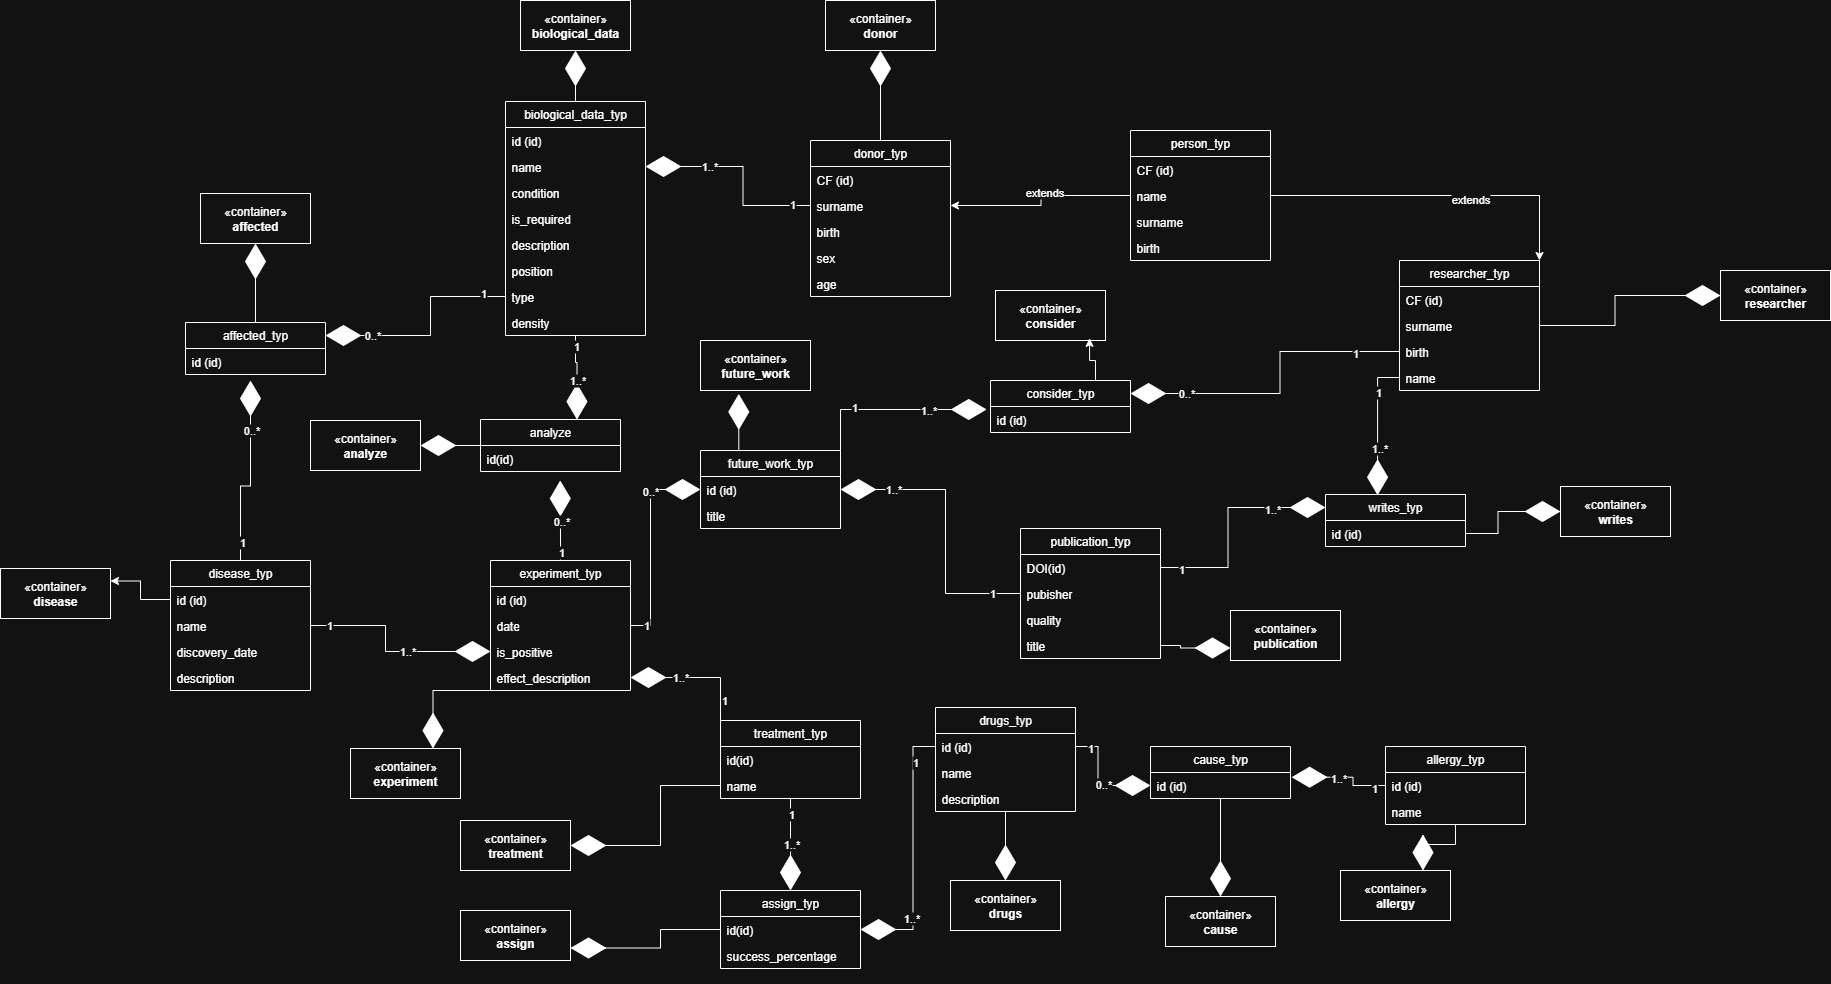
\includegraphics[width=1.10\textwidth]{img/UML progetto.drawio.png}
\caption{UML class diagram for the object–relational logical schema}
\label{fig:uml-logical}
\end{figure}

\section{Physical Design}

In this section, we discuss the physical design of our system, where the types defined in the logical and UML schemas are implemented in Oracle using object types, object tables, and association tables. This step translates the abstract entities and relationships into concrete physical structures that support persistence and efficient querying.

\subsection{Person hierarchy}
\begin{sqlbox}[title={PERSON\_TYP, DONOR\_TYP, RESEARCHER\_TYP}]
CREATE OR REPLACE TYPE person_typ AS OBJECT (
  CF        CHAR(16),
  name      VARCHAR2(100),
  surname   VARCHAR2(100),
  birth     DATE
) NOT FINAL;
/

CREATE OR REPLACE TYPE donor_typ UNDER person_typ (
  sex CHAR(1),
  age NUMBER(3)
);
/

CREATE OR REPLACE TYPE researcher_typ UNDER person_typ ();
/

CREATE TABLE donors_tab OF donor_typ (
  CF PRIMARY KEY
) OBJECT IDENTIFIER IS PRIMARY KEY;

CREATE TABLE researchers_tab OF researcher_typ (
  CF PRIMARY KEY
) OBJECT IDENTIFIER IS PRIMARY KEY;
\end{sqlbox}

We define a general type \texttt{person\_typ} as the supertype, capturing the attributes common to all persons. Two subtypes, \texttt{donor\_typ} and \texttt{researcher\_typ}, extend this base type with their specific details. Typed tables \texttt{donors\_tab} and \texttt{researchers\_tab} store the instances, with primary keys defined on the unique identifier CF.

\subsection{Entities}
\begin{sqlbox}{DISEASE\_TYP}
CREATE OR REPLACE TYPE disease_typ AS OBJECT (
  id              NUMBER,
  name            VARCHAR2(200),
  discovery_date  DATE,
  description     CLOB
);
/

CREATE TABLE disease_tab OF disease_typ (
  id PRIMARY KEY
) OBJECT IDENTIFIER IS PRIMARY KEY;
\end{sqlbox}

Diseases are represented as a standalone type with a corresponding object table.

\begin{sqlbox}{BIOLOGICAL\_DATA\_TYP}
CREATE OR REPLACE TYPE biological_data_typ AS OBJECT (
  id            NUMBER,
  name          VARCHAR2(200),
  condition     VARCHAR2(200),
  is_required   CHAR(1),
  description   CLOB,
  position      VARCHAR2(100),
  data_type     VARCHAR2(100),
  density       NUMBER,
  donor_ref     REF donor_typ
);
/

CREATE TABLE biological_data_tab OF biological_data_typ (
  id PRIMARY KEY,
  donor_ref NOT NULL,
  SCOPE FOR (donor_ref) IS donors_tab
) OBJECT IDENTIFIER IS PRIMARY KEY;
\end{sqlbox}

Biological data are modeled as a type containing attributes describing tissues and organs, with a \texttt{REF} to the donor. The typed table enforces referential integrity via the \texttt{SCOPE} clause.

\begin{sqlbox}{EXPERIMENT\_TYP}
CREATE OR REPLACE TYPE experiment_typ AS OBJECT (
  id                   NUMBER,
  exper_date           DATE,
  is_positive          CHAR(1),
  effect_description   VARCHAR2(1000),
  disease_ref          REF disease_typ,
  treatment_ref        REF treatment_typ
);
/

CREATE TABLE experiment_tab OF experiment_typ (
  id PRIMARY KEY,
  disease_ref NOT NULL,
  treatment_ref NOT NULL,
  SCOPE FOR (disease_ref) IS disease_tab,
  SCOPE FOR (treatment_ref) IS treatment_tab
) OBJECT IDENTIFIER IS PRIMARY KEY;
\end{sqlbox}

Experiments are linked to both diseases and treatments through \texttt{REF}s.

\begin{sqlbox}{TREATMENT\_TYP}
CREATE OR REPLACE TYPE treatment_typ AS OBJECT (
  id                  NUMBER,
  name                VARCHAR2(200),
  success_percentage  NUMBER(5,2)
);
/

CREATE TABLE treatment_tab OF treatment_typ (
  id PRIMARY KEY,
  name NOT NULL,
  success_percentage NOT NULL
) OBJECT IDENTIFIER IS PRIMARY KEY;
\end{sqlbox}

Experiments reference the treatment they apply; the treatment stores the overall \texttt{success\_percentage} for its drug combination.

\begin{sqlbox}{DRUGS\_TYP}
CREATE OR REPLACE TYPE drugs_typ AS OBJECT (
  id          NUMBER,
  name        VARCHAR2(200),
  description CLOB
);
/

CREATE TABLE drugs_tab OF drugs_typ (
  id PRIMARY KEY
) OBJECT IDENTIFIER IS PRIMARY KEY;
\end{sqlbox}

\begin{sqlbox}{ALLERGY\_TYP}
CREATE OR REPLACE TYPE allergy_typ AS OBJECT (
  id    NUMBER,
  name  VARCHAR2(200)
);
/

CREATE TABLE allergy_tab OF allergy_typ (
  id PRIMARY KEY
) OBJECT IDENTIFIER IS PRIMARY KEY;
\end{sqlbox}

Drugs and allergies are both modeled as object types with dedicated tables, allowing reuse and avoiding redundancy. The relationship between them is modeled separately as an association.

\subsection{Publications and Future Works}
\begin{sqlbox}{PUBLICATION\_TYP}
CREATE OR REPLACE TYPE publication_typ AS OBJECT (
  DOI        VARCHAR2(120),
  publisher  VARCHAR2(200),
  quality    VARCHAR2(50),
  title      VARCHAR2(300)
);
/

CREATE TABLE publication_tab OF publication_typ (
  DOI PRIMARY KEY
) OBJECT IDENTIFIER IS PRIMARY KEY;
\end{sqlbox}

\begin{sqlbox}{FUTURE\_WORK\_TYP}
CREATE OR REPLACE TYPE future_work_typ AS OBJECT (
  id        NUMBER,
  title     VARCHAR2(300),
  exp_ref   REF experiment_typ,
  pub_ref   REF publication_typ
);
/

CREATE TABLE future_work_tab OF future_work_typ (
  id PRIMARY KEY,
  exp_ref NOT NULL,
  pub_ref NOT NULL,
  SCOPE FOR (exp_ref) IS experiment_tab,
  SCOPE FOR (pub_ref) IS publication_tab
) OBJECT IDENTIFIER IS PRIMARY KEY;
\end{sqlbox}

Publications and future works are implemented as separate object types. Future works hold references to both experiments and publications.

\subsection{Association types and tables}
Many-to-many relationships from the conceptual schema are mapped to association types and stored in dedicated tables. Each table scopes its \texttt{REF}s to the appropriate target tables. Pair-wise uniqueness is enforced with triggers.

\begin{sqlbox}{ASSIGN\_TYP}
CREATE OR REPLACE TYPE assign_typ AS OBJECT (
  id             NUMBER,
  treatment_ref  REF treatment_typ,
  drug_ref       REF drugs_typ
);
/

CREATE TABLE assign_tab OF assign_typ (
  id PRIMARY KEY,
  treatment_ref NOT NULL,
  drug_ref NOT NULL,
  SCOPE FOR (treatment_ref) IS treatment_tab,
  SCOPE FOR (drug_ref) IS drugs_tab
) OBJECT IDENTIFIER IS PRIMARY KEY;
\end{sqlbox}

The \texttt{assign\_tab} table represents the many-to-many relationship between treatments and drugs.

\begin{sqlbox}{CAUSE\_TYP}
CREATE OR REPLACE TYPE cause_typ AS OBJECT (
  id           NUMBER,
  drug_ref     REF drugs_typ,
  allergy_ref  REF allergy_typ
);
/

CREATE TABLE cause_tab OF cause_typ (
  id PRIMARY KEY,
  drug_ref NOT NULL,
  allergy_ref NOT NULL,
  SCOPE FOR (drug_ref) IS drugs_tab,
  SCOPE FOR (allergy_ref) IS allergy_tab
) OBJECT IDENTIFIER IS PRIMARY KEY;
\end{sqlbox}

The \texttt{cause\_tab} table models the association between drugs and allergies.

\begin{sqlbox}{ANALYZE\_TYP}
CREATE OR REPLACE TYPE analyze_typ AS OBJECT (
  id        NUMBER,
  bio_ref   REF biological_data_typ,
  exp_ref   REF experiment_typ
);
/

CREATE TABLE analyze_tab OF analyze_typ (
  id PRIMARY KEY,
  bio_ref NOT NULL,
  exp_ref NOT NULL,
  SCOPE FOR (bio_ref) IS biological_data_tab,
  SCOPE FOR (exp_ref) IS experiment_tab
) OBJECT IDENTIFIER IS PRIMARY KEY;
\end{sqlbox}

The \texttt{analyze\_tab} table records which biological data have been analyzed in which experiments.

\begin{sqlbox}{AFFECTED\_TYP}
CREATE OR REPLACE TYPE affected_typ AS OBJECT (
  id           NUMBER,
  bio_ref      REF biological_data_typ,
  disease_ref  REF disease_typ
);
/

CREATE TABLE affected_tab OF affected_typ (
  id PRIMARY KEY,
  bio_ref NOT NULL,
  disease_ref NOT NULL,
  SCOPE FOR (bio_ref) IS biological_data_tab,
  SCOPE FOR (disease_ref) IS disease_tab
) OBJECT IDENTIFIER IS PRIMARY KEY;
\end{sqlbox}

The \texttt{affected\_tab} table models the association between biological data and diseases.

\begin{sqlbox}{WRITES\_TYP}
CREATE OR REPLACE TYPE writes_typ AS OBJECT (
  id               NUMBER,
  publication_ref  REF publication_typ,
  researcher_ref   REF researcher_typ
);
/

CREATE TABLE writes_tab OF writes_typ (
  id PRIMARY KEY,
  publication_ref NOT NULL,
  researcher_ref NOT NULL,
  SCOPE FOR (publication_ref) IS publication_tab,
  SCOPE FOR (researcher_ref) IS researchers_tab
) OBJECT IDENTIFIER IS PRIMARY KEY;
\end{sqlbox}

\begin{sqlbox}{CONSIDER\_TYP}
CREATE OR REPLACE TYPE consider_typ AS OBJECT (
  id               NUMBER,
  future_work_ref  REF future_work_typ,
  researcher_ref   REF researcher_typ
);
/

CREATE TABLE consider_tab OF consider_typ (
  id PRIMARY KEY,
  future_work_ref NOT NULL,
  researcher_ref NOT NULL,
  SCOPE FOR (future_work_ref) IS future_work_tab,
  SCOPE FOR (researcher_ref) IS researchers_tab
) OBJECT IDENTIFIER IS PRIMARY KEY;
\end{sqlbox}

The \texttt{writes\_tab} and \texttt{consider\_tab} tables represent the associations between researchers and their publications or future works.

\subsection{Check constraints (enumerations and ranges)}

We enforce value domains and basic ranges using CHECK constraints directly on the typed tables.

\begin{sqlbox}[title={Enumerations and ranges (BR1, BR2, BR3, BR4, BR6, BR7, BR8)}]
-- BR1: BiologicalData.condition in {control, disease}
ALTER TABLE biological_data_tab
  ADD CONSTRAINT chk_bd_condition
  CHECK (LOWER(condition) IN ('control','disease'));

-- BR3: BiologicalData.is_required in {Y,N}
ALTER TABLE biological_data_tab
  ADD CONSTRAINT chk_bd_is_required
  CHECK (UPPER(is_required) IN ('Y','N'));

-- BR2: BiologicalData.data_type in {organ, tissue}
ALTER TABLE biological_data_tab
  ADD CONSTRAINT chk_bd_data_type
  CHECK (LOWER(data_type) IN ('organ','tissue'));

-- BR8: BiologicalData.density > 0
ALTER TABLE biological_data_tab
  ADD CONSTRAINT chk_bd_density_pos
  CHECK (density > 0);

-- BR4: Experiment.is_positive in {Y,N}
ALTER TABLE experiment_tab
  ADD CONSTRAINT chk_experiment_is_positive
  CHECK (UPPER(is_positive) IN ('Y','N'));

-- BR6: Treatment.success_percentage integer in [0,100]
ALTER TABLE treatment_tab
  ADD CONSTRAINT chk_treatment_success
  CHECK (success_percentage BETWEEN 0 AND 100 AND success_percentage = TRUNC(success_percentage));

-- BR7: Publication.quality in {top,middle,low}
ALTER TABLE publication_tab
  ADD CONSTRAINT chk_publication_quality
  CHECK (LOWER(quality) IN ('top','middle','low'));
\end{sqlbox}

These constraints are lightweight, declarative, and push invalid data out early without procedural code.

\subsection{Triggers}

This subsection documents the triggers used to enforce business rules and cross-entity consistency in the Oracle physical schema. Each code box shows the exact DDL, followed by a short rationale.

\begin{sqlbox}[title={Temporal consistency for diseases and experiments (BR12, BR13)}]
-- BR12: Experiment.exper_date \>= Disease.discovery_date
CREATE OR REPLACE TRIGGER trg_experiment_date_vs_disease
BEFORE INSERT OR UPDATE OF exper_date, disease_ref ON experiment_tab
FOR EACH ROW
DECLARE
  v_discovery_date DATE;
BEGIN
  SELECT d.discovery_date INTO v_discovery_date
  FROM disease_tab d
  WHERE REF(d) = :NEW.disease_ref;

  IF :NEW.exper_date < v_discovery_date THEN
    RAISE_APPLICATION_ERROR(-20001, 'Experiment date must be on or after the Disease discovery_date');
  END IF;
END;
/

-- BR13: Disease.discovery_date must not be in the future
CREATE OR REPLACE TRIGGER trg_disease_discovery_not_future
BEFORE INSERT OR UPDATE OF discovery_date ON disease_tab
FOR EACH ROW
BEGIN
  IF :NEW.discovery_date > SYSDATE THEN
    RAISE_APPLICATION_ERROR(-20002, 'Disease discovery_date cannot be in the future');
  END IF;
END;
/
\end{sqlbox}

These triggers guarantee temporal sanity: experiments cannot predate the discovery of the disease they attempt; diseases cannot be discovered in the future.

\begin{sqlbox}{Biological Data condition and Affected consistency (BR9)}
-- Allow Affected only if BD.condition = 'disease'
CREATE OR REPLACE TRIGGER trg_affected_insert_check_condition
BEFORE INSERT OR UPDATE OF bio_ref ON affected_tab
FOR EACH ROW
DECLARE
  v_condition VARCHAR2(200);
BEGIN
  SELECT b.condition INTO v_condition FROM biological_data_tab b WHERE REF(b) = :NEW.bio_ref;
  IF LOWER(v_condition) <> 'disease' THEN
    RAISE_APPLICATION_ERROR(-20003, 'Affected link allowed only for BiologicalData with condition = disease');
  END IF;
END;
/

-- Prevent deleting the last Affected when BD is diseased
CREATE OR REPLACE TRIGGER trg_affected_prevent_delete_last
BEFORE DELETE ON affected_tab
FOR EACH ROW
DECLARE
  v_condition VARCHAR2(200);
  v_cnt NUMBER;
BEGIN
  SELECT b.condition INTO v_condition FROM biological_data_tab b WHERE REF(b) = :OLD.bio_ref;
  IF LOWER(v_condition) = 'disease' THEN
    SELECT COUNT(*) INTO v_cnt
    FROM affected_tab a
    WHERE a.bio_ref = :OLD.bio_ref
      AND NOT (a.bio_ref = :OLD.bio_ref AND a.disease_ref = :OLD.disease_ref);
    IF v_cnt = 0 THEN
      RAISE_APPLICATION_ERROR(-20004, 'Cannot delete the last Affected row for a diseased BiologicalData');
    END IF;
  END IF;
END;
/

-- Forbid setting condition=control if Affected links exist
CREATE OR REPLACE TRIGGER trg_bd_condition_change
BEFORE UPDATE OF condition ON biological_data_tab
FOR EACH ROW
DECLARE
  v_cnt NUMBER;
BEGIN
  IF LOWER(:NEW.condition) = 'control' THEN
    SELECT COUNT(*) INTO v_cnt
    FROM affected_tab a
    WHERE a.bio_ref = (SELECT REF(b) FROM biological_data_tab b WHERE b.id = :NEW.id);
    IF v_cnt > 0 THEN
      RAISE_APPLICATION_ERROR(-20010, 'Cannot set condition=control while Affected links exist');
    END IF;
  END IF;
END;
/
\end{sqlbox}

These three triggers keep \texttt{Biological Data} and \texttt{Affected} coherent with the stated semantics of control vs diseased samples.

\begin{sqlbox}{Future Work requires a positive Experiment}
-- By assumption, only useful Future Works are created; enforce positivity of the source experiment
CREATE OR REPLACE TRIGGER trg_future_work_requires_positive_exp
BEFORE INSERT OR UPDATE OF exp_ref ON future_work_tab
FOR EACH ROW
DECLARE
  v_is_pos CHAR(1);
BEGIN
  SELECT e.is_positive INTO v_is_pos FROM experiment_tab e WHERE REF(e) = :NEW.exp_ref;
  IF UPPER(v_is_pos) <> 'Y' THEN
    RAISE_APPLICATION_ERROR(-20011, 'FutureWork requires a positive Experiment');
  END IF;
END;
/
\end{sqlbox}

\noindent\textbf{Uniqueness on REF pairs with compound triggers.} REF columns do not support direct UNIQUE constraints; moreover, row-level checks would require selecting from the same table being modified, which leads to mutating-table issues during multi-row statements. We therefore adopted compound triggers that collect the key pairs in the \textit{BEFORE EACH ROW} phase and validate duplicates only \textit{AFTER STATEMENT}.

\begin{sqlbox}{Compound uniqueness on REF pairs (example: Affected)}
-- Representative example: uniqueness (bio_ref, disease_ref) on AFFECTED via a compound trigger
CREATE OR REPLACE TRIGGER trg_aff_uni
FOR INSERT OR UPDATE OF bio_ref, disease_ref ON affected_tab
COMPOUND TRIGGER
  TYPE pair_rec IS RECORD (bio_id NUMBER, disease_id NUMBER);
  TYPE pair_tab IS TABLE OF pair_rec INDEX BY PLS_INTEGER;
  g_pairs pair_tab; g_idx PLS_INTEGER := 0;

  PROCEDURE add_pair(p_b REF biological_data_typ, p_d REF disease_typ) IS
    v_b NUMBER; v_d NUMBER;
  BEGIN
    SELECT b.id INTO v_b FROM biological_data_tab b WHERE REF(b) = p_b;
    SELECT d.id INTO v_d FROM disease_tab d       WHERE REF(d) = p_d;
    g_idx := g_idx + 1; g_pairs(g_idx).bio_id := v_b; g_pairs(g_idx).disease_id := v_d;
  END;

  BEFORE EACH ROW IS
  BEGIN
    IF INSERTING OR UPDATING THEN
      add_pair(:NEW.bio_ref, :NEW.disease_ref);
    END IF;
  END BEFORE EACH ROW;

  AFTER STATEMENT IS
    v_cnt NUMBER;
  BEGIN
    FOR i IN 1..g_idx LOOP
      SELECT COUNT(*) INTO v_cnt
      FROM affected_tab a
      WHERE DEREF(a.bio_ref).id = g_pairs(i).bio_id
        AND DEREF(a.disease_ref).id = g_pairs(i).disease_id;
      IF v_cnt > 1 THEN
        RAISE_APPLICATION_ERROR(-20030, 'Duplicate Affected (bio,disease)');
      END IF;
    END LOOP;
  END AFTER STATEMENT;
END;
/
\end{sqlbox}

The same pattern applies to the other association tables with REF pairs (\texttt{analyze\_tab}, \texttt{assign\_tab}, \texttt{cause\_tab}, \texttt{writes\_tab}, \texttt{consider\_tab}); only the identifiers and the error message differ.

\begin{sqlbox}{Analyze vs Disease consistency (BR14)}
-- On Analyze insert/update, BD must be diseased and match Experiment.disease
CREATE OR REPLACE TRIGGER trg_analyze_consistency
BEFORE INSERT OR UPDATE OF bio_ref, exp_ref ON analyze_tab
FOR EACH ROW
DECLARE
  v_condition VARCHAR2(200);
  v_cnt NUMBER;
BEGIN
  SELECT b.condition INTO v_condition FROM biological_data_tab b WHERE REF(b) = :NEW.bio_ref;
  IF LOWER(v_condition) = 'control' THEN
    RAISE_APPLICATION_ERROR(-20005, 'Control BiologicalData cannot be analyzed in experiments attempting a disease');
  END IF;

  SELECT COUNT(*) INTO v_cnt
  FROM affected_tab a
  WHERE a.bio_ref = :NEW.bio_ref
    AND a.disease_ref = (SELECT e.disease_ref FROM experiment_tab e WHERE REF(e) = :NEW.exp_ref);
  IF v_cnt = 0 THEN
    RAISE_APPLICATION_ERROR(-20006, 'BiologicalData must be affected by the same disease attempted by the Experiment');
  END IF;
END;
/

-- Prevent removing Affected if Analyze rows rely on it
CREATE OR REPLACE TRIGGER trg_affected_block_if_analyze_exists
BEFORE DELETE ON affected_tab
FOR EACH ROW
DECLARE
  v_cnt NUMBER;
BEGIN
  SELECT COUNT(*) INTO v_cnt
  FROM analyze_tab z
  WHERE z.bio_ref = :OLD.bio_ref
    AND EXISTS (
      SELECT 1 FROM experiment_tab e
      WHERE REF(e) = z.exp_ref
        AND e.disease_ref = :OLD.disease_ref
    );
  IF v_cnt > 0 THEN
    RAISE_APPLICATION_ERROR(-20007, 'Cannot remove Affected: existing Analyze rows require this disease link');
  END IF;
END;
/
\end{sqlbox}

Together, these triggers ensure that each analyzed sample is affected by the exact disease attempted by the linked experiment and that the dependency is preserved.

---

In conclusion, the physical design translates the conceptual entities into object types and typed tables. Association entities are modeled as separate types and tables to correctly represent many-to-many relationships while avoiding redundancy. This design balances normalization, reuse of objects, and performance considerations, ensuring an efficient mapping between the logical schema and its physical implementation.

\subsection{Operations}

This subsection documents how the five main operations are implemented at the physical level. We provide one stored procedure per operation. Read-oriented procedures return a \texttt{SYS\_REFCURSOR} to stream results; the insert-oriented procedure commits on success following the course examples.

\begin{sqlbox}{OP1 — Recording an organ or tissue}
-- Insert a Biological Data (organ/tissue) for a given donor
CREATE OR REPLACE PROCEDURE proc_record_biological_data (
  p_id           IN NUMBER,
  p_name         IN VARCHAR2,
  p_condition    IN VARCHAR2,   -- 'control' | 'disease'
  p_is_required  IN CHAR,       -- 'Y' | 'N'
  p_description  IN CLOB,
  p_position     IN VARCHAR2,
  p_data_type    IN VARCHAR2,   -- 'organ' | 'tissue'
  p_density      IN NUMBER,
  p_donor_cf     IN CHAR
) AS
  v_donor_ref REF donor_typ;
BEGIN
  SELECT REF(d) INTO v_donor_ref FROM donors_tab d WHERE d.CF = p_donor_cf;
  INSERT INTO biological_data_tab
  VALUES (biological_data_typ(p_id, p_name, p_condition, p_is_required,
                              p_description, p_position, p_data_type,
                              p_density, v_donor_ref));
  COMMIT;
EXCEPTION
  WHEN NO_DATA_FOUND THEN
    RAISE_APPLICATION_ERROR(-20020, 'Donor not found for provided CF');
  WHEN OTHERS THEN
    RAISE_APPLICATION_ERROR(-20021, 'Error in proc_record_biological_data: ' || SQLERRM);
END;
/ 
\end{sqlbox}

\begin{sqlbox}{OP2 — Organs/tissues below a density threshold}
-- Return: id, name, data_type, density, donor_cf, is_required, condition
CREATE OR REPLACE PROCEDURE proc_list_bio_below_density (
  p_threshold IN NUMBER,
  p_result    OUT SYS_REFCURSOR
) AS
BEGIN
  OPEN p_result FOR
    SELECT b.id,
           b.name,
           b.data_type,
           b.density,
           DEREF(b.donor_ref).CF AS donor_cf,
           b.is_required,
           b.condition
      FROM biological_data_tab b
     WHERE b.density < p_threshold;
EXCEPTION
  WHEN OTHERS THEN
    RAISE_APPLICATION_ERROR(-20022, 'Error in proc_list_bio_below_density: ' || SQLERRM);
END;
/ 
\end{sqlbox}

\begin{sqlbox}{OP3 — Treatment info with drugs and linked allergies}
-- One row per (drug, allergy) combination, with treatment details
CREATE OR REPLACE PROCEDURE proc_get_treatment_info (
  p_treatment_id IN NUMBER,
  p_result       OUT SYS_REFCURSOR
) AS
BEGIN
  OPEN p_result FOR
    SELECT t.id                      AS treatment_id,
           t.name                    AS treatment_name,
           t.success_percentage,
           d.id                      AS drug_id,
           d.name                    AS drug_name,
           al.id                     AS allergy_id,
           al.name                   AS allergy_name
      FROM treatment_tab t
      LEFT JOIN assign_tab a
             ON a.treatment_ref = REF(t)
      LEFT JOIN drugs_tab d
             ON a.drug_ref = REF(d)
      LEFT JOIN cause_tab c
             ON c.drug_ref = a.drug_ref
      LEFT JOIN allergy_tab al
             ON c.allergy_ref = REF(al)
       WHERE t.id = p_treatment_id;
EXCEPTION
  WHEN OTHERS THEN
    RAISE_APPLICATION_ERROR(-20023, 'Error in proc_get_treatment_info: ' || SQLERRM);
END;
/ 
\end{sqlbox}

\begin{sqlbox}{OP4 — Donors with a given disease on life-required BD and useful FWs}
-- Distinct donors (CF, name, surname) for a disease name, only if BD is required for life
-- and at least one Future Work exists via Analyze → Experiment
CREATE OR REPLACE PROCEDURE proc_list_donors_required_disease_with_fw (
  p_disease_name IN VARCHAR2,
  p_result       OUT SYS_REFCURSOR
) AS
BEGIN
  OPEN p_result FOR
    SELECT DISTINCT d.CF,
                    d.name,
                    d.surname
      FROM donors_tab d
      JOIN biological_data_tab b
        ON b.donor_ref = REF(d)
      JOIN affected_tab a
        ON a.bio_ref = REF(b)
      JOIN disease_tab dis
        ON a.disease_ref = REF(dis)
       AND LOWER(dis.name) = LOWER(p_disease_name)
     WHERE LOWER(b.condition) = 'disease'
       AND UPPER(b.is_required) = 'Y'
       AND EXISTS (
             SELECT 1
               FROM analyze_tab z
               JOIN future_work_tab f
                 ON f.exp_ref = z.exp_ref
              WHERE z.bio_ref = REF(b)
            );
EXCEPTION
  WHEN OTHERS THEN
    RAISE_APPLICATION_ERROR(-20024, 'Error in proc_list_donors_required_disease_with_fw: ' || SQLERRM);
END;
/ 
\end{sqlbox}

\begin{sqlbox}{OP5 — Useful suggestions sent to researchers with top-quality pubs}
-- Return: future work id, title, and researcher identity
CREATE OR REPLACE PROCEDURE proc_list_fw_for_top_researchers (
  p_result OUT SYS_REFCURSOR
) AS
BEGIN
  OPEN p_result FOR
    SELECT
      f.id      AS future_work_id,
      f.title   AS future_work_title,
      r.CF      AS researcher_cf,
      r.name    AS researcher_name,
      r.surname AS researcher_surname
    FROM consider_tab c
    JOIN future_work_tab f
      ON c.future_work_ref = REF(f)
    JOIN (
        SELECT DISTINCT w.researcher_ref
        FROM writes_tab w
        JOIN publication_tab p
          ON w.publication_ref = REF(p)
        WHERE p.quality = 'top'
    ) top_researchers
      ON c.researcher_ref = top_researchers.researcher_ref
    JOIN researchers_tab r
      ON c.researcher_ref = REF(r);
EXCEPTION
  WHEN OTHERS THEN
    RAISE_APPLICATION_ERROR(-20025, 'Error in proc_list_fw_for_top_researchers: ' || SQLERRM);
END;
/ 
\end{sqlbox}

\subsection{Indexes}

\textbf{Qualitative assessment.} In this paragraph we will choose specific indexes based on the type of operation to be performed and the way Oracle accesses data.

\subsubsection*{OP2}

The operation retrieves all biological data (organs / tissues) whose density is below a threshold. Since the attribute is numerical and the operation involves a range predicate, a B+Tree index is the most appropriate choice: it supports efficient range scans, whereas hash-based indexing would only be suitable for exact equality lookups.  

\begin{figure}[H]
  \centering
  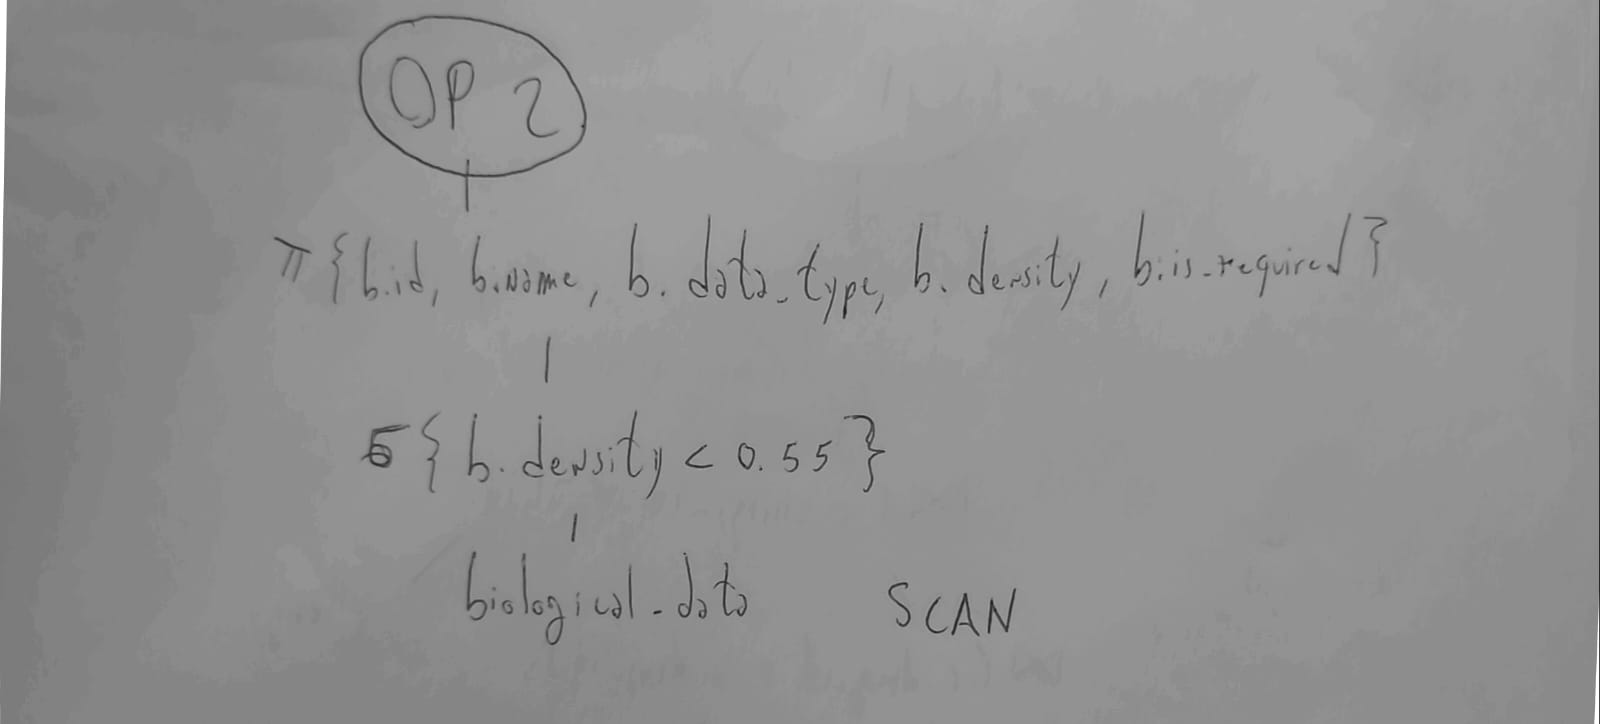
\includegraphics[width=0.8\textwidth]{img/op2_algebra.png}
  \caption{Algebraic tree of OP2}
\end{figure}

\textbf{Initial analysis (no index).} Autotrace shows a full table scan on \texttt{BIOLOGICAL\_DATA\_TAB}, which is expected because the optimizer has no auxiliary structure to exploit. This implies a cost that grows linearly with the table size.  

We then created a B+Tree index:  

\begin{sqlbox}
CREATE INDEX idx_bd_density ON biological_data_tab(density);
\end{sqlbox}

\textbf{After adding the index.} The access path changes to an INDEX RANGE SCAN with Table Access by ROWID. The complexity becomes logarithmic in the blocking factor, offering stable performance as the table grows.  

\begin{figure}[H]
  \centering
  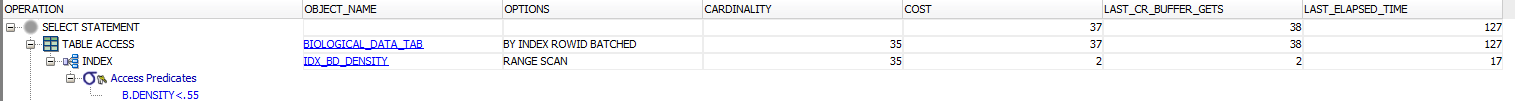
\includegraphics[width=0.8\textwidth]{img/op2_autotrace_after.png}
  \caption{Autotrace of OP2 after adding the index}
\end{figure}

\textit{Alternative.} One might consider a hash index or hash cluster, but this would only benefit equality predicates. Since our query uses a range condition (\(< 0.55\)), the B+Tree is unequivocally the better option.

\subsubsection*{OP3}

The operation retrieves treatment details and associated drugs/allergies. Logically it follows a chain of joins starting from the treatment primary key. Since the entry point is already indexed by the PK, the challenge is optimizing the association tables (\texttt{ASSIGN\_TAB} and \texttt{CAUSE\_TAB}).  

\begin{figure}[H]
  \centering
  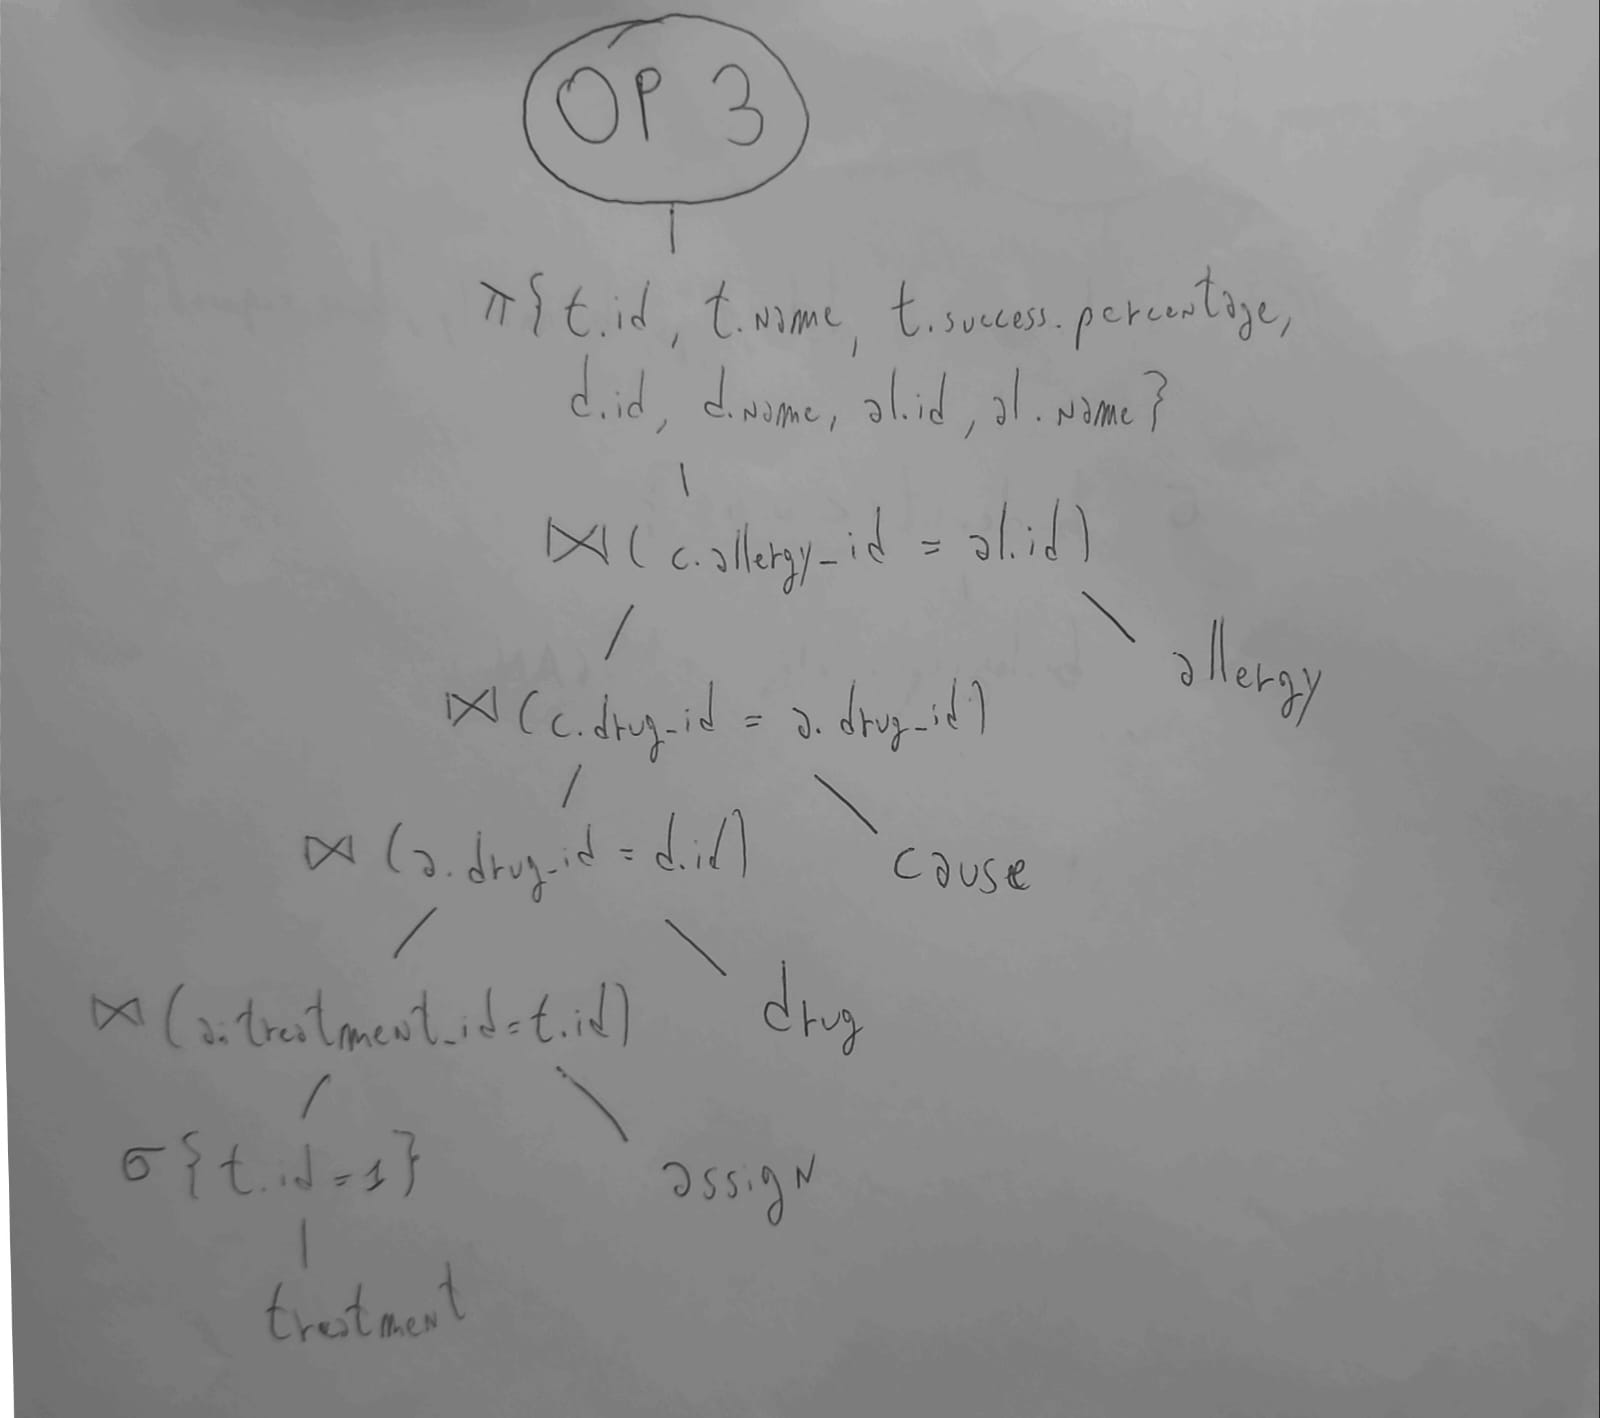
\includegraphics[width=0.8\textwidth]{img/op3_algebra.png}
  \caption{Algebraic tree of OP3}
\end{figure}

\textbf{Initial analysis (no auxiliary indexes).} Autotrace shows full scans on the association tables. With the current small dataset, this is not too expensive, but it will not scale when the tables grow.  

After analyzing the query execution plan, we create B+Tree indexes only on the REF columns that are actually utilized by Oracle's optimizer:

\begin{sqlbox}
CREATE INDEX idx_assign_treatment_ref ON assign_tab(treatment_ref);
CREATE INDEX idx_cause_drug_ref       ON cause_tab(drug_ref);
\end{sqlbox}

\textbf{Rationale for index selection.} These two indexes are sufficient because:
\begin{itemize}
    \item \texttt{idx\_assign\_treatment\_ref} — enables efficient access when joining \texttt{treatment\_tab} to \texttt{assign\_tab}
    \item \texttt{idx\_cause\_drug\_ref} — enables efficient access when joining from \texttt{assign\_tab} to \texttt{cause\_tab}
\end{itemize}

Additional indexes on \texttt{assign\_tab(drug\_ref)} or \texttt{cause\_tab(allergy\_ref)} would be redundant since:
\begin{itemize}
    \item The join from \texttt{assign\_tab} to \texttt{drugs\_tab} is efficiently served by the primary key index on \texttt{drugs\_tab}
    \item The join from \texttt{cause\_tab} to \texttt{allergy\_tab} benefits from the primary key index on \texttt{allergy\_tab}
\end{itemize}

This minimal indexing strategy reduces storage overhead and maintenance cost while providing optimal query performance.

\begin{figure}[H]
  \centering
  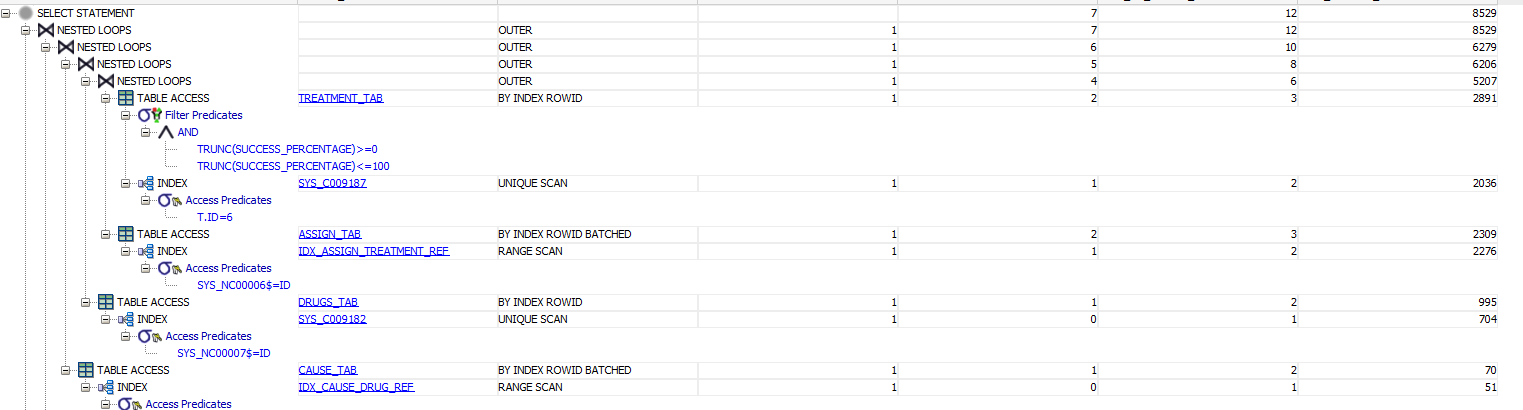
\includegraphics[width=0.8\textwidth]{img/op3_autotrace_after.png}
  \caption{Autotrace of OP3 after adding the indexes}
\end{figure}

\subsubsection*{OP4}

The query selects donors affected by a given disease and linked (through experiments) to future work entries. It therefore traverses multiple association tables.  

\begin{figure}[H]
  \centering
  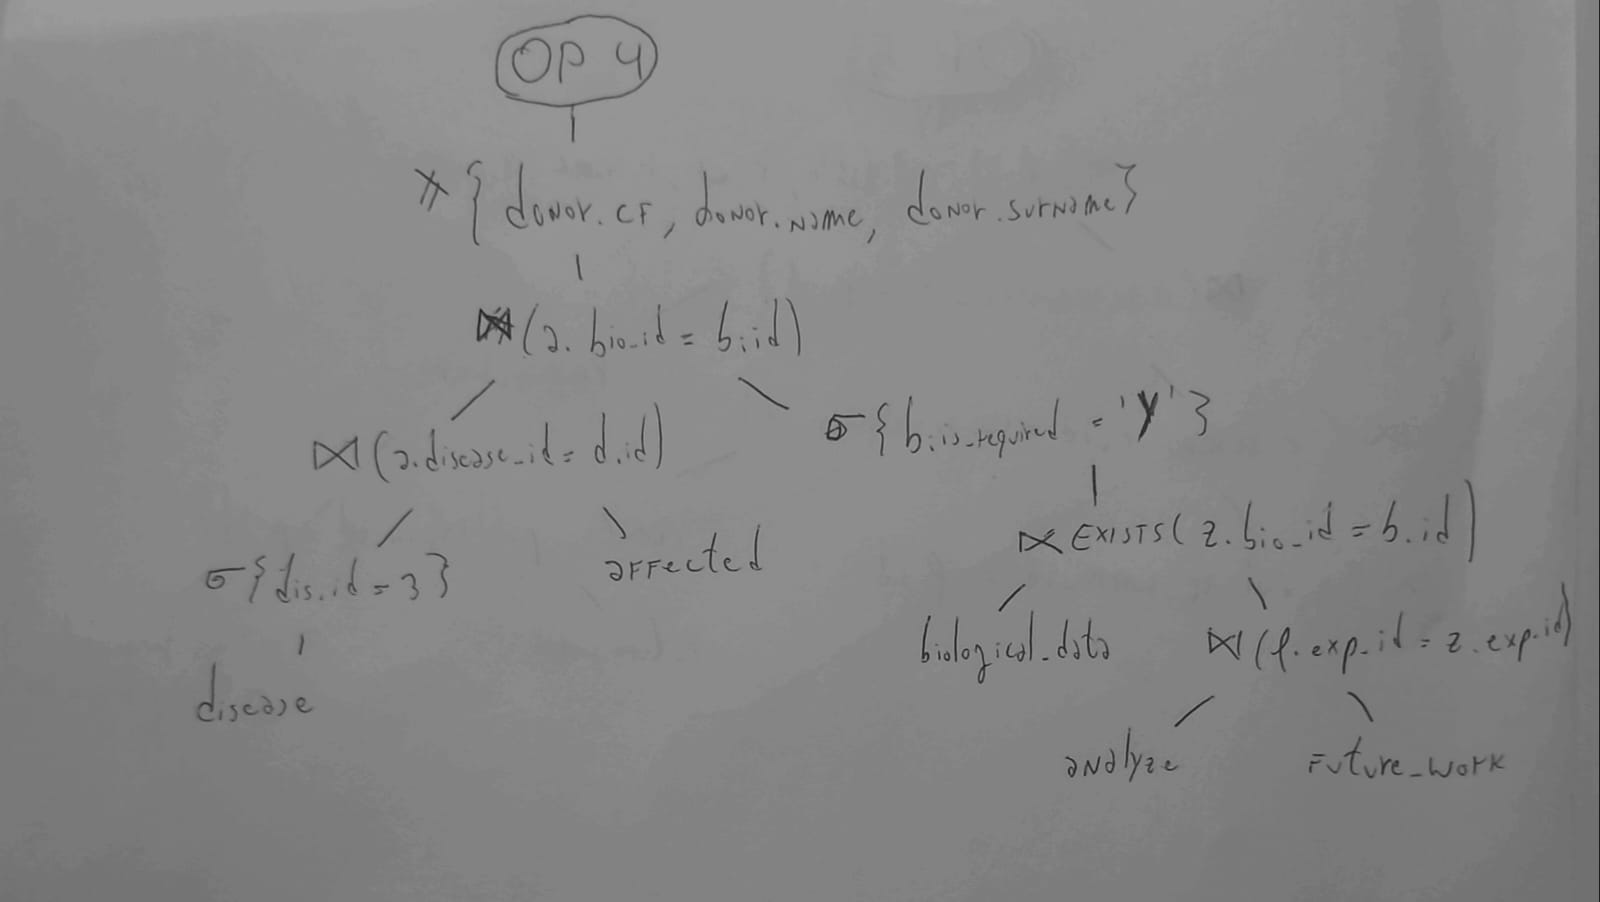
\includegraphics[width=0.8\textwidth]{img/op4_algebra.png}
  \caption{Algebraic tree of OP4}
\end{figure}

\textbf{Initial analysis (no index).} Autotrace showed several FULL SCANs (on \texttt{AFFECTED\_TAB}, \texttt{ANALYZE\_TAB}, \texttt{FUTURE\_WORK\_TAB}). This leads to a high number of logical reads, proportional to the size of these tables.  

To optimize, we created narrow B+Tree indexes targeting the selective joins:  

\begin{sqlbox}
CREATE INDEX idx_aff_dis_bio ON affected_tab(disease_ref, bio_ref);
CREATE INDEX idx_analyze_bio ON analyze_tab(bio_ref);
CREATE INDEX idx_fw_exp      ON future_work_tab(exp_ref);
\end{sqlbox}

\textbf{Rationale for index selection:}
\begin{itemize}
    \item \texttt{idx\_aff\_dis\_bio} — composite index enabling efficient lookup by disease and biological data
    \item \texttt{idx\_analyze\_bio} — critical for the EXISTS subquery join condition \texttt{z.bio\_ref = REF(b)}, eliminates FULL SCAN on \texttt{analyze\_tab} when dataset is sufficiently large
    \item \texttt{idx\_fw\_exp} — used in the EXISTS subquery to find future works linked to experiments
\end{itemize}

\textbf{Note on optimizer behavior:} With small datasets, Oracle may prefer FULL SCAN over index access due to lower overhead. After increasing the dataset size (12K biological data, 15K experiments, 18K future works), Oracle correctly uses \texttt{idx\_analyze\_bio} for index range scans.

\textbf{After adding the indexes.} Oracle now exploits index-driven nested loops. The FULL SCAN on \texttt{analyze\_tab} is eliminated, replaced by index range scans. Logical gets are reduced significantly, and the plan shows efficient index access on all join columns.

\begin{figure}[H]
  \centering
  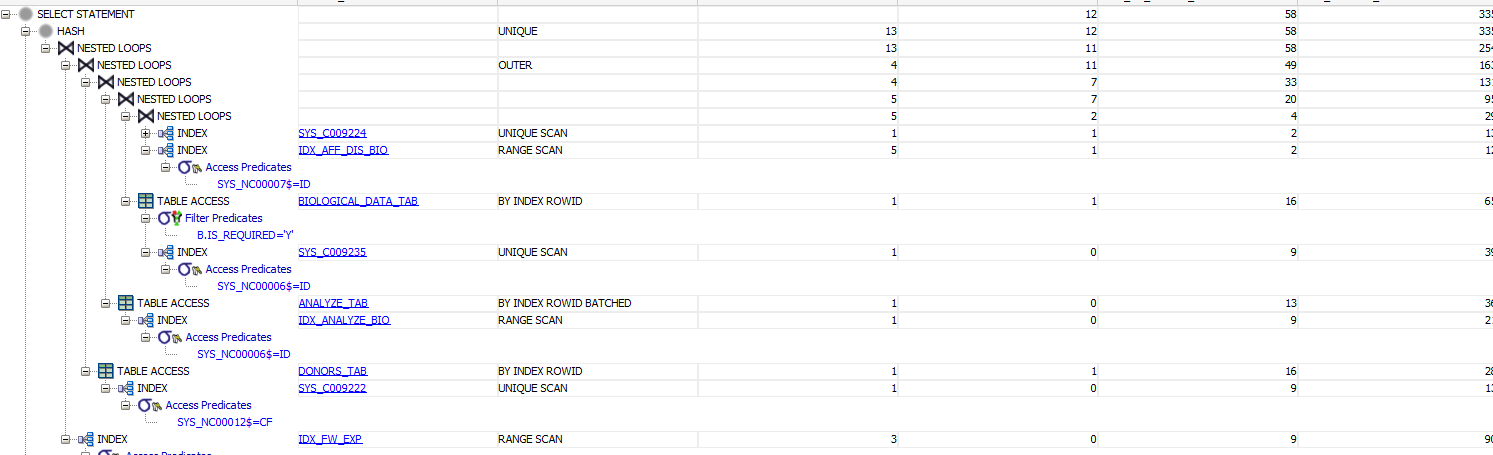
\includegraphics[width=0.8\textwidth]{img/op4_autotrace_after.png}
  \caption{Autotrace of OP4 after adding the indexes}
\end{figure}

\subsubsection*{OP5}

This operation retrieves all \texttt{Future Work} entries considered by researchers with at least one high-quality publication. The query filters on \texttt{PUBLICATION\_TAB} and then joins \texttt{WRITES\_TAB} and \texttt{CONSIDER\_TAB}.  

\begin{figure}[H]
  \centering
  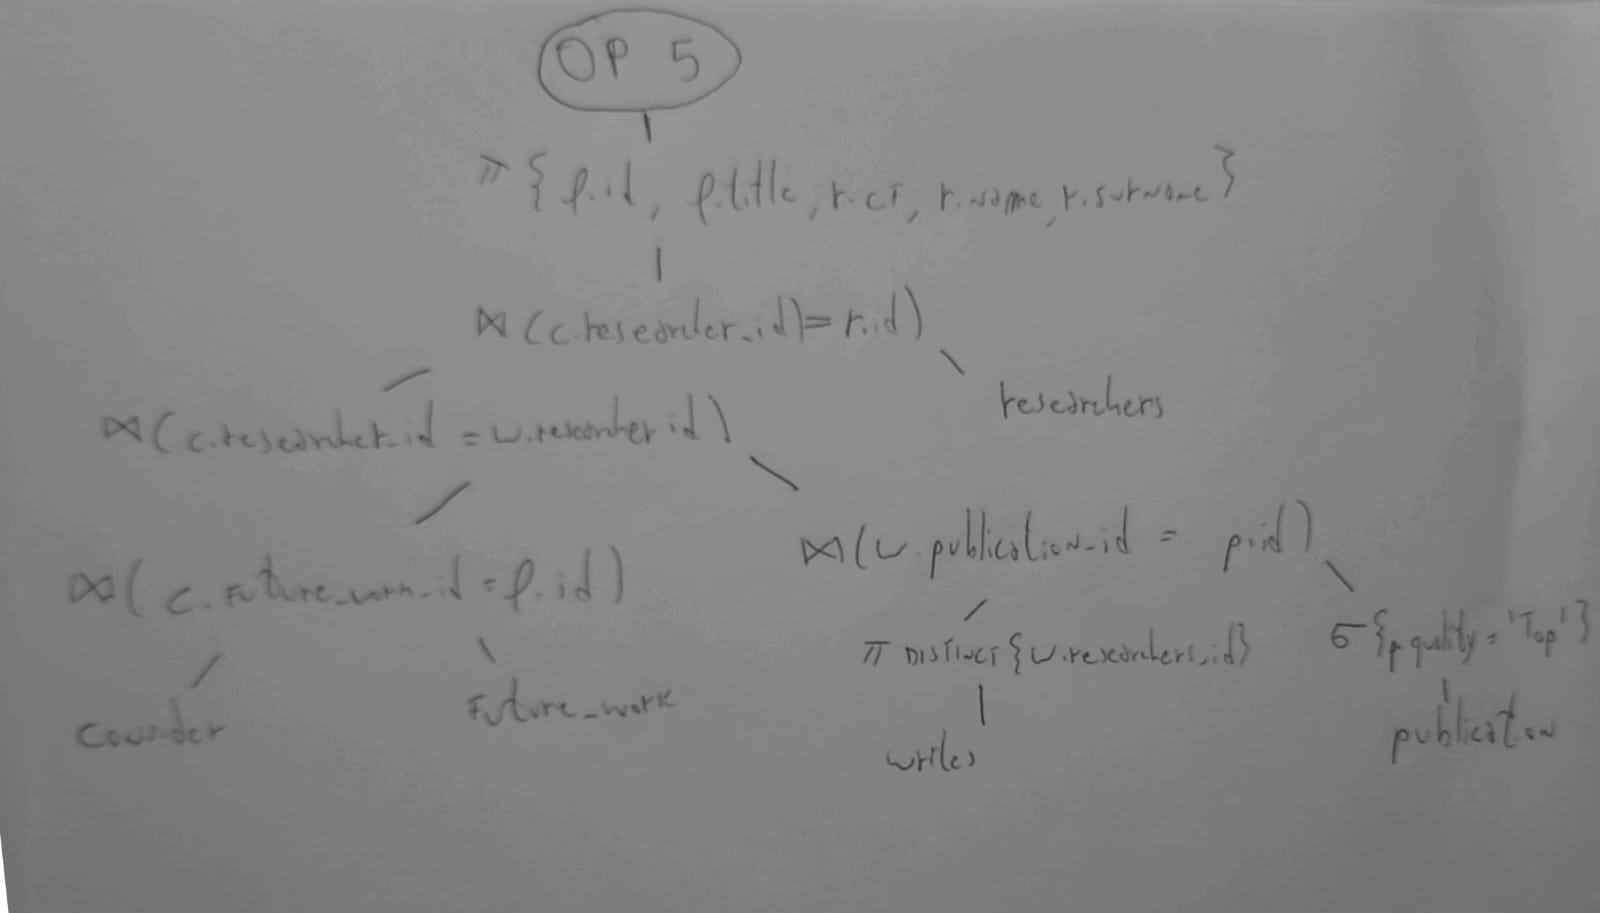
\includegraphics[width=0.8\textwidth]{img/op5_algebra.png}
  \caption{Algebraic tree of OP5}
\end{figure}

\textbf{Initial analysis (no index).} Autotrace showed full scans on the publication and association tables, combined with hash joins. While functional, this approach scales poorly because each join requires scanning entire tables, regardless of selectivity.  

We created B+Tree indexes on the most selective columns to optimize join operations:

\begin{sqlbox}
CREATE INDEX idx_pub_quality         ON publication_tab(quality);
CREATE INDEX idx_writes_publication_ref  ON writes_tab(publication_ref);
CREATE INDEX idx_consider_researcher_ref ON consider_tab(researcher_ref);
\end{sqlbox}

\textbf{Rationale for index selection:}
\begin{itemize}
    \item \texttt{idx\_pub\_quality} — enables efficient filtering on \texttt{quality = 'top'} to find high-quality publications, reducing the workload during the initial scan
    \item \texttt{idx\_writes\_publication\_ref} — used for the join from \texttt{publication\_tab} to \texttt{writes\_tab}, avoiding a full table scan on \texttt{writes\_tab}
    \item \texttt{idx\_consider\_researcher\_ref} — critical for joining the researcher subquery with \texttt{consider\_tab}, significantly reducing the scan cost on this association table
\end{itemize}

\textbf{After adding the indexes.} Autotrace confirms that Oracle correctly uses all three indexes:
\begin{itemize}
    \item \texttt{idx\_pub\_quality} performs an INDEX RANGE SCAN on \texttt{publication\_tab}, filtering only the top-quality publications
    \item \texttt{idx\_writes\_publication\_ref} performs an INDEX RANGE SCAN on \texttt{writes\_tab}, efficiently joining publications to their authors
    \item \texttt{idx\_consider\_researcher\_ref} performs an INDEX RANGE SCAN on \texttt{consider\_tab}, efficiently joining researchers to their assigned future works
\end{itemize}

These indexes significantly reduce the execution cost by eliminating full table scans on the association tables and enabling selective access to the publication table. The cost-based optimizer leverages these indexes to construct an efficient execution plan with nested loop joins instead of expensive hash joins on full table scans. Note that \texttt{researchers\_tab} and \texttt{future\_work\_tab} still use FULL TABLE SCAN.

\begin{figure}[H]
  \centering
  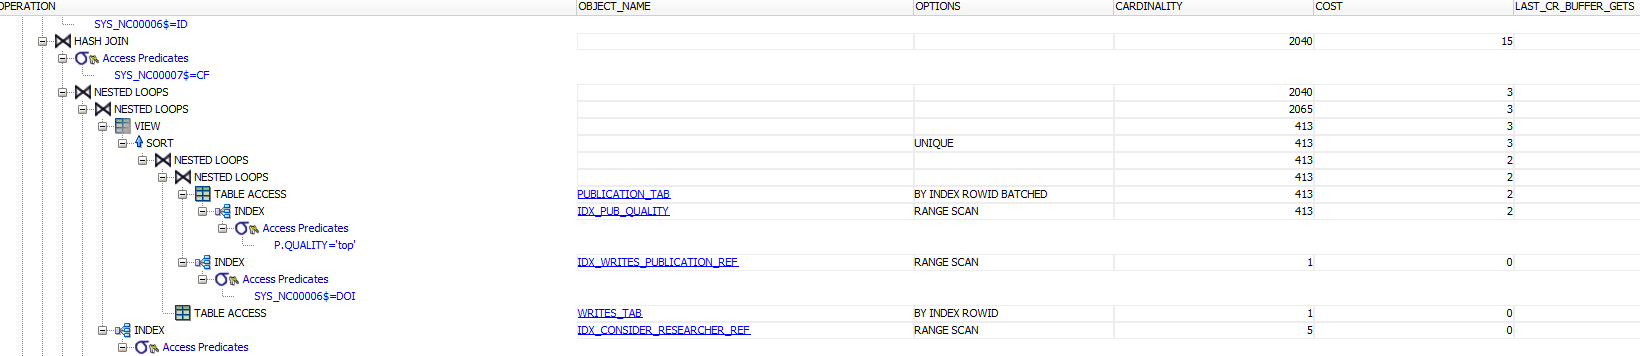
\includegraphics[width=0.8\textwidth]{img/op5_autotrace_after.png}
  \caption{Autotrace of OP5 after adding the indexes}
\end{figure}

\subsubsection*{General note on index choice}

Hash indexes (or hash clusters) can be advantageous only for \emph{equality} queries on well-distributed, relatively static data. In our context this is not the case: most attributes are queried with ranges or through joins, the data distribution is not uniform, and the system undergoes constant updates (insertion of new experiments, publications, future works, etc.). These factors would increase the cost of hash structures and risk collisions. Moreover, since the operations are executed only once a month, it is not justified to create specialized auxiliary structures with limited usage. For these reasons, B+Tree indexes remain the most appropriate choice, as they provide both flexibility and stability across different query patterns.

\section{Web Application}

The web application provides a user-friendly interface to interact with the WHO Disease Monitoring System. It allows users to visualize stored data, insert new records, and execute the 5 analytical operations previously described.

\subsection{Technology Stack and Architecture}

The application is built using:
\begin{itemize}
    \item \textbf{Flask}: Python 3.11 web framework for routing and request handling
    \item \textbf{oracledb}: Oracle database driver
    \item \textbf{Docker}: Containerization for portability and ease of deployment
\end{itemize}


\subsection{Database Interaction}

\paragraph{Connection Management}
The application establishes connections to Oracle Database using the \texttt{oracledb} library:
\begin{sqlbox}{python}
def get_db_connection():
    connection = oracledb.connect(
        user=Config.DB_USER,
        password=Config.DB_PASSWORD,
        dsn=Config.get_dsn()
    )
    return connection
\end{sqlbox}

\paragraph{Data Visualization and Insertion}
The webapp provides interfaces to:
\begin{itemize}
    \item \textbf{List} all records from each entity table (Biological Data, Donor, Disease, Treatment, Drug, Allergy, Experiment, Future Work, Publication, Researcher)
    \item \textbf{Insert} new records with proper form validation and business rule enforcement
    \item Manage association tables (Affected, Analyze, Assign, Cause, Consider, Write) with dynamic filtering to prevent constraint violations
\end{itemize}

For example, the \texttt{Analyze} form implements client-side JavaScript filtering to ensure BR14 compliance: when a user selects a biological data sample, the experiment dropdown automatically shows only experiments attempting to treat the same disease affecting that sample.

\paragraph{Analytical Operations with Stored Procedures}
To maintain business logic entirely within the database layer, all 5 analytical operations are implemented as Oracle \textbf{stored procedures}. This approach ensures that complex queries and data processing logic remain in the database, while the application layer handles only presentation and user interaction.

For each operation, custom Oracle object types define the return structure. For example, Operation 2 uses:
\begin{sqlbox}{sql}
CREATE TYPE op2_result_typ AS OBJECT (
    bio_id NUMBER,
    bio_name VARCHAR2(100),
    density NUMBER,
    position VARCHAR2(200),
    donor_name VARCHAR2(50),
    donor_surname VARCHAR2(50)
);

CREATE TYPE op2_result_tab AS TABLE OF op2_result_typ;
\end{sqlbox}

The stored procedure encapsulates the entire query logic:
\begin{sqlbox}{sql}
CREATE OR REPLACE FUNCTION func_list_bio_below_density(
    p_threshold NUMBER
) RETURN op2_result_tab PIPELINED IS
BEGIN
    FOR rec IN (
        SELECT b.id, b.name, b.density, b.position,
               DEREF(b.donor).name AS donor_name,
               DEREF(b.donor).surname AS donor_surname
        FROM biological_data_tab b
        WHERE b.density < p_threshold
        ORDER BY b.density
    ) LOOP
        PIPE ROW(op2_result_typ(rec.id, rec.name, 
                 rec.density, rec.position,
                 rec.donor_name, rec.donor_surname));
    END LOOP;
    RETURN;
END;
\end{sqlbox}

The Flask application invokes the stored procedure using standard SQL syntax:
\begin{sqlbox}{python}
@app.route('/operations/2', methods=['GET', 'POST'])
def operation_2():
    if request.method == 'POST':
        threshold = float(request.form.get('threshold'))
        cursor.execute("""
            SELECT * FROM TABLE(
                func_list_bio_below_density(:threshold)
            )
        """, {'threshold': threshold})
        results = cursor.fetchall()
        return render_template('operation_2.html', 
                             results=results)
    return render_template('operation_2.html')
\end{sqlbox}

This pattern is replicated for all operations:

This pattern is replicated for all operations:
\begin{itemize}
    \item \textbf{Operation 2}: \texttt{func\_list\_bio\_below\_density(threshold)} — Lists biological data below a specified density threshold
    \item \textbf{Operation 3}: \texttt{func\_get\_treatment\_info(treatment\_id)} — Retrieves treatment details with associated drugs and allergies
    \item \textbf{Operation 4}: \texttt{func\_list\_donors\_required\_disease\_with\_fw(disease\_id)} — Lists donors with a disease affecting vital organs for which useful future works were suggested
    \item \textbf{Operation 5}: \texttt{func\_list\_fw\_for\_top\_researchers()} — Lists useful future works assigned to researchers with top-quality publications
\end{itemize}

This architecture ensures:
\begin{itemize}
    \item All business logic resides in the database layer through PL/SQL stored procedures
    \item The application layer remains thin, handling only presentation and routing
    \item Query optimization and execution plans are managed by Oracle's query optimizer
\end{itemize}

\subsection{Deployment}

The application can be started with a single PowerShell command:
\begin{verbatim}
.\start.ps1
\end{verbatim}

This script orchestrates the entire deployment process:
\begin{enumerate}
    \item Builds Docker images for database and webapp services
    \item Starts containers in detached mode
    \item Waits for Oracle Database to be ready
    \item Initializes the schema with DDL scripts
    \item Loads sample data
    \item Deploys stored procedures for analytical operations
    \item Makes the application available at \texttt{http://localhost:5000}
\end{enumerate}

The \texttt{.\textbackslash stop.ps1} script gracefully shuts down all services and removes the containers.

\subsection{User Interface Examples}

The following figures illustrate key pages of the web application.

\begin{figure}[H]
  \centering
  \fbox{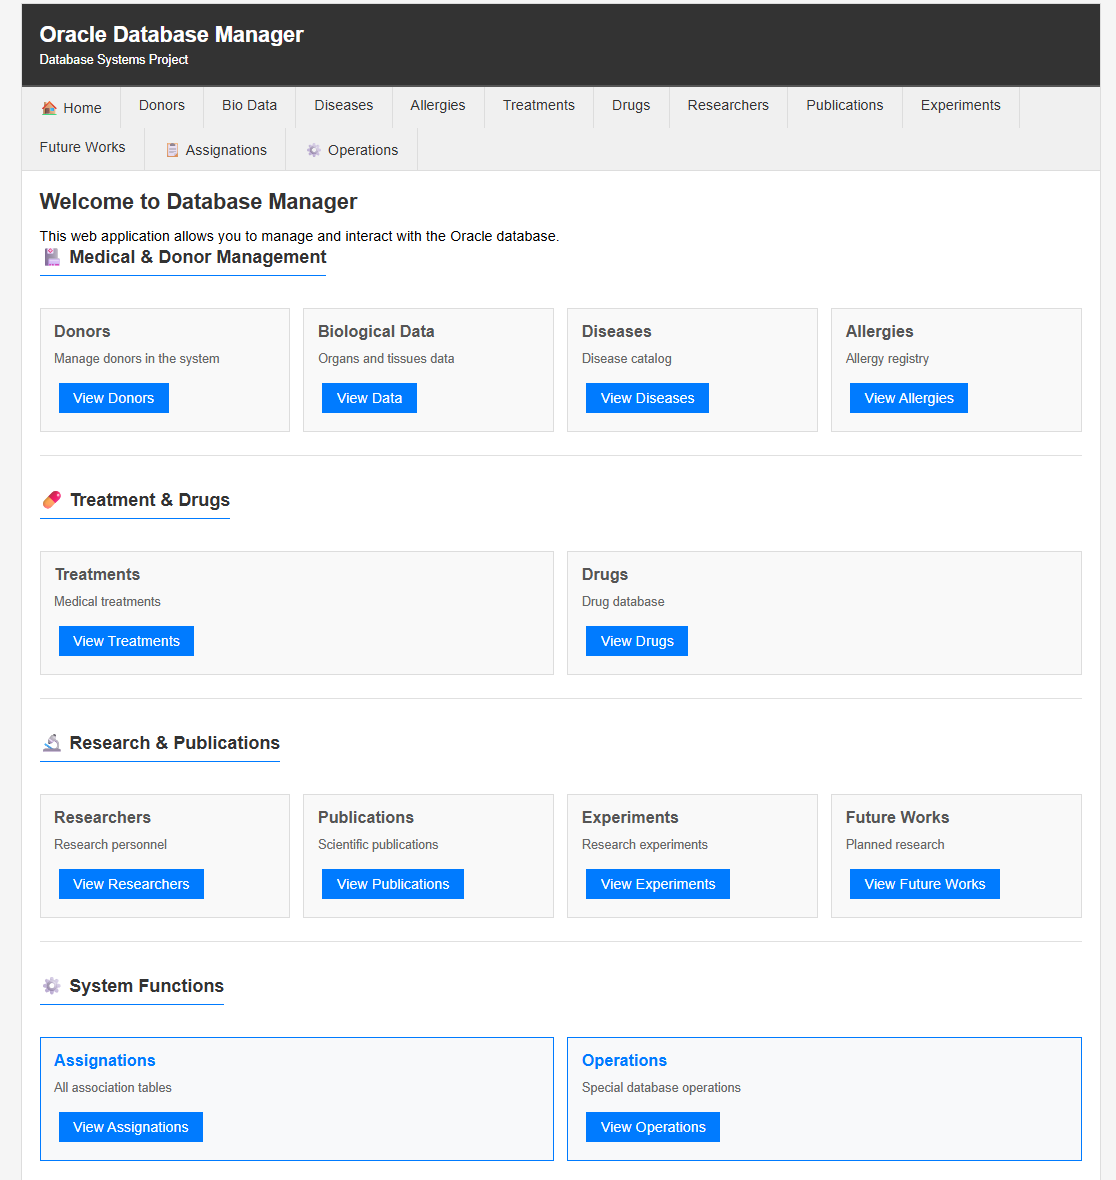
\includegraphics[width=0.85\textwidth]{img/webapp_home.png}}
  \caption{Homepage with navigation menu to all entities and operations}
  \label{fig:webapp-home}
\end{figure}

\begin{figure}[H]
  \centering
  \fbox{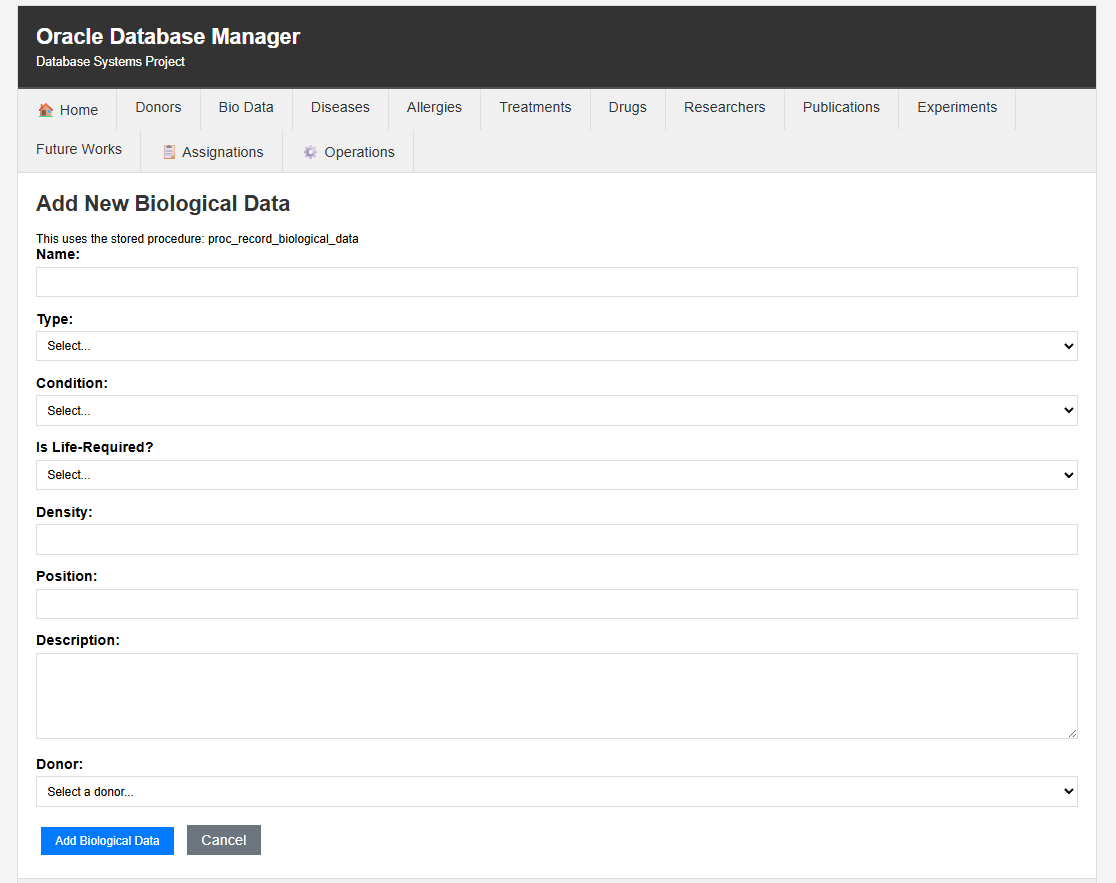
\includegraphics[width=0.85\textwidth]{img/webapp_add_biological_data.png}}
  \caption{Form for adding new biological data (organ or tissue)}
  \label{fig:webapp-add-bio}
\end{figure}

\begin{figure}[H]
  \centering
  \fbox{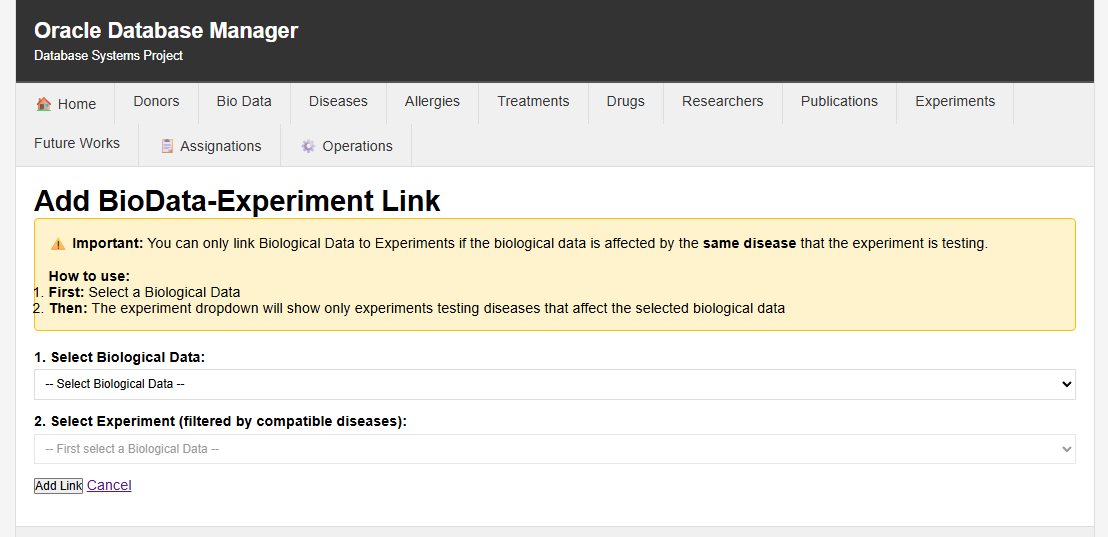
\includegraphics[width=0.85\textwidth]{img/webapp_analyze_dynamic.png}}
  \caption{Dynamic filtering in Analyze form: experiment dropdown filtered by biological data disease}
  \label{fig:webapp-analyze}
\end{figure}

\begin{figure}[H]
  \centering
  \fbox{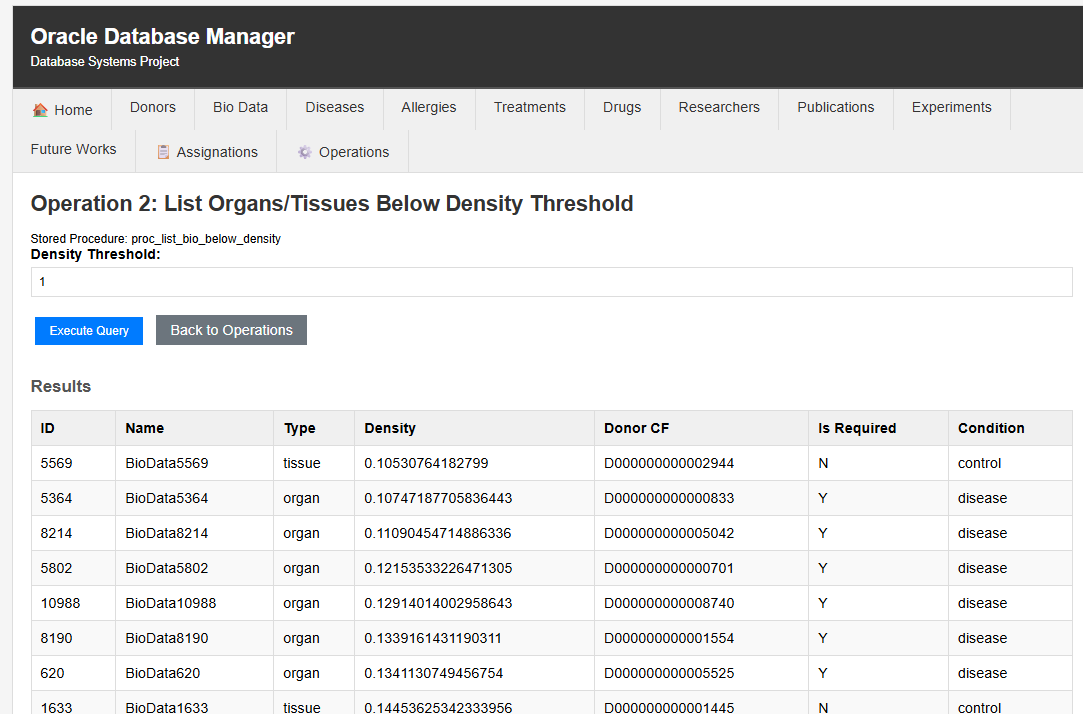
\includegraphics[width=0.85\textwidth]{img/webapp_operation2.png}}
  \caption{Operation 2: List biological data below density threshold}
  \label{fig:webapp-op2}
\end{figure}

\begin{figure}[H]
  \centering
  \fbox{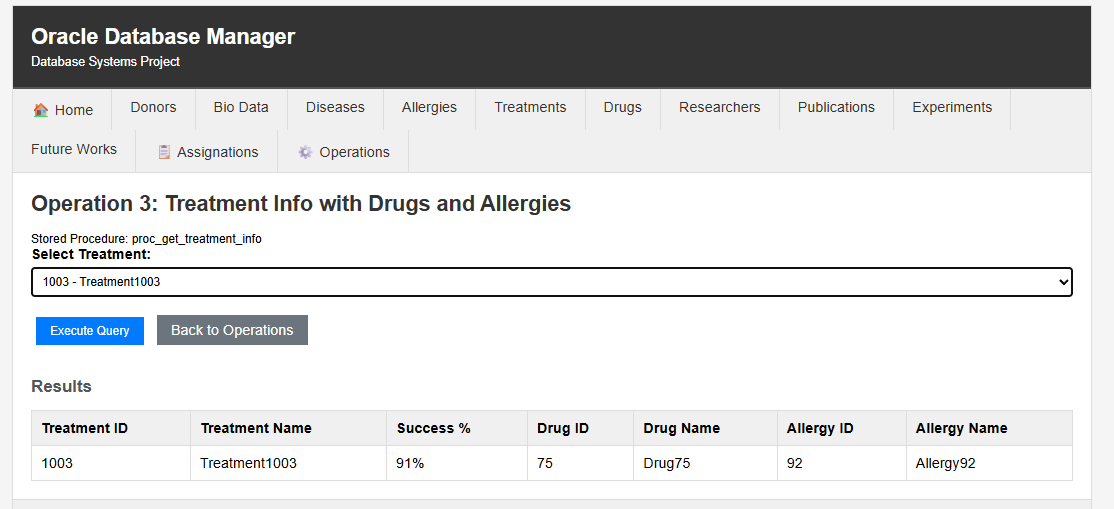
\includegraphics[width=0.85\textwidth]{img/webapp_operation3.png}}
  \caption{Operation 3: Treatment details with associated drugs and allergies}
  \label{fig:webapp-op3}
\end{figure}

The web application successfully demonstrates the practical applicability of the designed database system, providing an accessible interface for WHO personnel to manage disease monitoring data effectively.

\section{Data Warehouse Design}

To support strategic decision-making and analytical processing, we propose a Data Warehouse design for the WHO Disease Monitoring System. This Data Warehouse will enable multidimensional analysis of key performance indicators, facilitating long-term trend analysis and evidence-based research planning.

\subsection{Fact and Dimension Analysis}

The analysis of facts, measures, and dimensions led to the definition of two key facts: \textbf{Disease Research Progress} and \textbf{Scientific Publication Output}. The need to analyze disease research progress arises from the goal of evaluating treatment effectiveness and predicting which diseases are closest to finding cures, enabling the WHO to allocate resources efficiently. Scientific publication output, on the other hand, will be analyzed to evaluate research productivity and ensure the organization maintains its reputation for high-quality scientific contributions.

\subsubsection{Fact 1: Disease Research Progress}

For Disease Research Progress, the dimensions considered will be Time, Disease, Treatment, Biological Data, and Area. The reasons for selecting these dimensions are:

\begin{itemize}
    \item \textbf{Time}: Helps identify research trends and predict future progress based on historical patterns of experiment success rates.
    
    \item \textbf{Disease}: Allows understanding which diseases are showing research progress and which require additional investment, enabling targeted resource allocation.
    
    \item \textbf{Treatment}: Identifies which treatments are most effective across different diseases, optimizing drug development strategies.
    
    \item \textbf{Biological Data}: Provides insights into whether organs or tissues, control or disease samples yield better experimental results, improving sample selection for future experiments.
    
    \item \textbf{Area}: Enables geographical analysis to study how geographic location impacts disease prevalence, treatment effectiveness, and research outcomes across different regions, continents, and countries.
\end{itemize}

\textbf{Measures:} numExperiments, successRate.

\subsubsection{Fact 2: Scientific Publication Output}

For Scientific Publication Output, the dimensions considered will be Time, Researcher, Publication, and Area.

\begin{itemize}
    \item \textbf{Time}: Tracks publication trends over time, helping to identify patterns in research productivity and assess output consistency.
    
    \item \textbf{Researcher}: Allows us to focus on researchers with lower publication rates or quality scores, identifying causes of underperformance and implementing targeted support programs.
    
    \item \textbf{Publication}: Helps understand publication quality distribution and publisher preferences, enabling the organization to improve overall publication standards and scientific impact.
    
    \item \textbf{Area}: Provides geographical insights into research productivity, allowing analysis of which regions produce more high-quality publications and identifying areas requiring additional research support.
\end{itemize}

\textbf{Measures:} numPublications, avgQualityScore.

\subsection{Schema Architecture}

The Data Warehouse will be implemented using a \textbf{Constellation Schema}. Specifically, this architecture is chosen because multiple dimensions are shared across different facts:

\begin{itemize}
    \item \textbf{Time dimension}: Shared by both facts to enable cross-fact temporal analysis and unified reporting across disease research and publication trends. Granularity includes Year, Month, Day for flexible time-based aggregations.
    
    \item \textbf{Area dimension}: Shared by both facts to enable geographical analysis of research impact, disease distribution, treatment effectiveness, and publication productivity across different regions, continents, and countries.
\end{itemize}

There are no issues with this sharing, as each fact maintains the same granularity for the shared dimensions.

The two fact tables are:

\begin{itemize}
    \item \textbf{ResearchProgress}: Links Time, Disease, Treatment, BiologicalData, and Area dimensions. Measures include numExperiments and successRate. Primary key: Time\_FK, Disease\_FK, Treatment\_FK, BiologicalData\_FK, Area\_FK.
    
    \item \textbf{PublicationOutput}: Links Time, Researcher, Publication, and Area dimensions. Measures include numPublications and avgQualityScore. Primary key: Time\_FK, Researcher\_FK, Publication\_FK, Area\_FK.
\end{itemize}

\begin{figure}[H]
  \centering
  \fbox{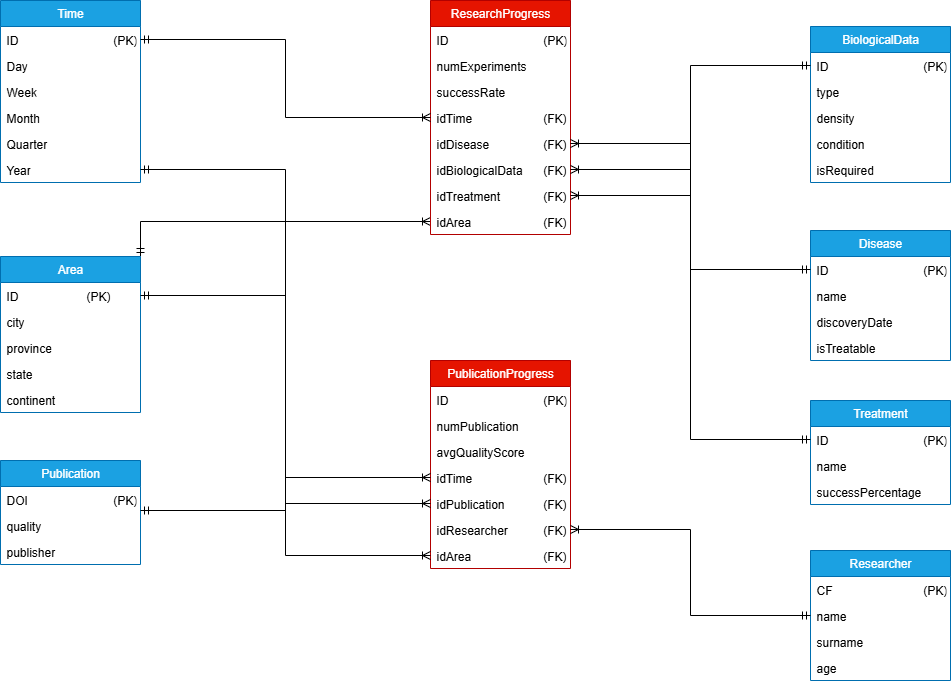
\includegraphics[width=0.95\textwidth]{img/dw_constellation_schema.png}}
  \caption{Constellation Schema for WHO Disease Monitoring Data Warehouse}
  \label{fig:dw-schema}
\end{figure}

\subsection{Summary}

The proposed Data Warehouse design provides the WHO with a powerful analytical platform for strategic decision-making. The two facts, Disease Research Progress and Scientific Publication Output, address the organization's core objectives of advancing medical research and maintaining scientific excellence. The constellation schema architecture ensures efficient data organization while enabling flexible multidimensional analysis across shared dimensions.


\end{document}
